\documentclass[12pt]{report}

\usepackage[language=english, type=bachelor]{style}
\usepackage{fancyhdr}
\usepackage{listings}
\usepackage{booktabs}
\usepackage{array}
\usepackage{tabularx}
\usepackage{pgfplots}
\usepackage{tikz}
\usepackage{xcolor}
\usepackage{xurl}

\geometry{a4paper,top=2.5cm,left=3cm,right=2.5cm,bottom=2.5cm}
\setlength{\emergencystretch}{3em}
\pgfplotsset{compat=1.18}
\usetikzlibrary{shapes.geometric, arrows.meta, positioning, fit, calc, matrix, backgrounds}

\definecolor{motivoBlue}{RGB}{37,99,235}
\definecolor{motivoCyan}{RGB}{8,145,178}
\definecolor{motivoGreen}{RGB}{22,163,74}
\definecolor{motivoAmber}{RGB}{217,119,6}
\definecolor{motivoRose}{RGB}{225,29,72}
\definecolor{motivoViolet}{RGB}{124,58,237}
\definecolor{motivoInk}{RGB}{30,41,59}
\definecolor{motivoSoft}{RGB}{241,245,249}

\lstdefinelanguage{Motivo}{
  morekeywords={
    tempo,signature,track,using,pattern,play,for,loop,if,else,let,from,voice,rest,true,false,piano,
    guitar,bass,violin,drums,kick,snare,hihat,crash,ride
  },
  sensitive=true,
  morecomment=[l]{//},
  morecomment=[s]{/*}{*/},
  morestring=[b]{"} % chktex 18
}
\lstset{
  basicstyle=\ttfamily\small,
  breaklines=true,
  columns=fullflexible,
  frame=single,
  rulecolor=\color{motivoInk!30},
  keywordstyle=\color{motivoBlue}\bfseries,
  commentstyle=\color{motivoGreen!70!black},
  stringstyle=\color{motivoRose},
  showstringspaces=false
}

\pagestyle{fancy}
\setlength{\headheight}{14.5pt}
\lhead{}
\chead{}
\renewcommand{\headrulewidth}{0.2pt}
\renewcommand{\footrulewidth}{0.2pt}

\begin{document}

\specialization{COMPUTER SCIENCE --- ENGLISH}
\title{Design and Implementation of a Domain-Specific Language for Music Composition}
\author{Moșneguțu Adrian-Ioan}
\supervisor{Dr.\ Lect.\ Mircea Ioan-Gabriel}

\hypersetup{pageanchor=false}
\maketitle

\newpage
\thispagestyle{empty}
\mbox{}
\newpage
\pagenumbering{roman}
\hypersetup{pageanchor=true}

ABSTRACT

\vspace{0.5cm}
\hrule
\vspace{0.5cm}

Digital audio workstations make detailed editing practical, but they store music as flat note events, so repetitive
structure is tedious to change and easy to lose.
Live-coding and scripting approaches recover programmability, yet they usually target real-time performance or
low-level event assembly rather than deterministic offline compilation to a portable score.

This thesis presents \textit{Motivo}, a domain-specific language and native compiler that keeps compositional structure
explicit in source and expands it into a Standard MIDI File without a language runtime at playback.
Motivo Studio wraps the toolchain in a browser-based editor for writing, compiling, and auditioning results.

We describe the language design, compiler implementation, studio application, and an empirical evaluation on synthetic
workloads.
The results support a bounded engineering claim: compact structural descriptions can be expanded into large timelines
within interactive compile times, without positioning Motivo as a replacement for established production tools.


\tableofcontents

\newpage
\pagenumbering{arabic}

\chapter{Research Context and Theoretical Foundations}\label{ch:context}

Music composition is both a creative activity and a structural one. A finished piece may be experienced as
sound, but during composition it is usually organized as motifs, repetitions, phrases, sections, instrumental
layers, tempo decisions, and symbolic note events. This thesis starts from that structural view of music. The
central question is not whether code should replace a digital audio workstation, a score editor, or a live
performance environment. The question is narrower: when a composer already thinks in terms of repeated
symbolic patterns, can a small compiled language make that structure explicit and produce a standard musical artifact?

The answer explored in this work is Motivo, a domain-specific language for offline symbolic composition.
Motivo is designed for situations where the desired output is a deterministic MIDI file rather than a live
audio stream. The language allows the composer to define patterns, tracks, voices, notes, rests, chords,
sequences, and control flow. The compiler then expands those structures into a timeline of MIDI note events.
The web application built around the compiler, Motivo Studio, provides the surrounding software engineering
layer: editing, diagnostics, visualization, playback, deployment, testing, and continuous integration.

This chapter combines motivation, theoretical background, and related work because the project is not a pure
theory contribution. It is a bachelor-level software engineering project informed by compiler construction,
music representation, and algorithmic composition. The chapter therefore follows the path of the problem:
first the growth of digital music workflows, then the limits of manual event editing, then the musical and
compiler concepts needed by the design, then the related systems that motivate Motivo's position.

\section{Digital Music as a Practical Software Domain}\label{sec:digital-music-domain}

Recorded music is now a large digital ecosystem rather than a niche computing topic.
IFPI reported that global recorded music revenues reached US\$31.7 billion in 2025, with streaming representing 69.6\%
of total recorded music revenue and paid subscription streaming representing 52.4\% of the total
market~\cite{IFPI_2026}.
Spotify, reporting from the perspective of a single streaming platform, stated that it paid more than US\$11 billion to
the music industry in 2025~\cite{Spotify_2026_Payouts}.
BandLab's public product material describes a community of 100 million music creators using its platform
ecosystem~\cite{BandLab_2026}.
These figures should not be read as a direct measurement of demand for a programming language.
They do, however, show that digital music creation, distribution, and consumption are large enough for specialized
creative software to be a relevant engineering topic.

\begin{figure}[htbp]
  \centering
  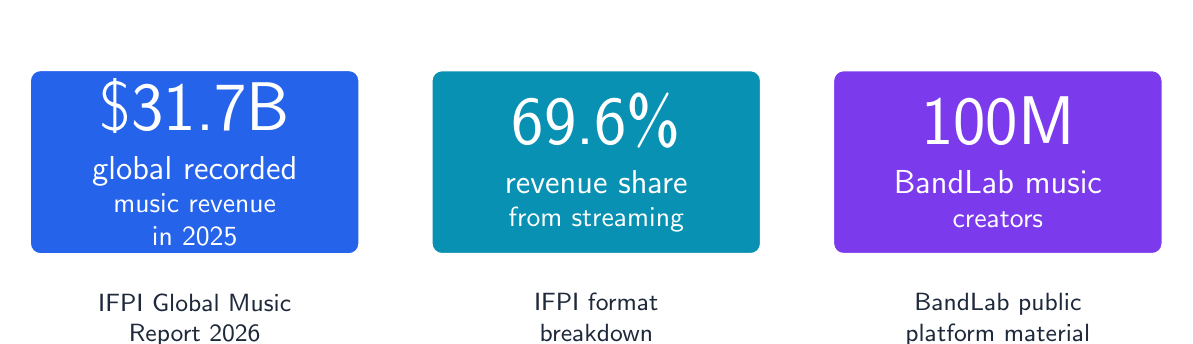
\begin{tikzpicture}[
      fact/.style={rounded corners=4pt, draw=white, very thick, minimum width=4.2cm, minimum height=2.35cm,
      align=center, font=\sffamily, text=white},
      caption/.style={font=\small\sffamily, text=motivoInk, align=center}
    ]
    \node[fact, fill=motivoBlue] (revenue) at (0, 0) {\Huge \$31.7B\\[0.2cm]\large global recorded\\music
    revenue\\in 2025};
    \node[fact, fill=motivoCyan] (streaming) at (5.1, 0) {\Huge 69.6\%\\[0.2cm]\large revenue share\\from streaming};
    \node[fact, fill=motivoViolet] (creators) at (10.2, 0) {\Huge 100M\\[0.2cm]\large BandLab music\\creators};

    \node[caption, below=0.35cm of revenue] {IFPI Global Music\\Report 2026};
    \node[caption, below=0.35cm of streaming] {IFPI format\\breakdown};
    \node[caption, below=0.35cm of creators] {BandLab public\\platform material};
  \end{tikzpicture}
  \caption{Industry-scale signals motivating digital music tooling.
    The numbers are attributed to their reporting organizations and are used as context, not as a direct evaluation of
  Motivo.}\label{fig:industry-context}
\end{figure}

The production side of this ecosystem is heavily tool-based.
Digital audio workstations make detailed editing possible through piano rolls, arrangement timelines, automation lanes,
plug-ins, and MIDI routing.
For many tasks this visual approach is the right interface.
It is direct, immediate, and close to the way a composer hears a piece.
At the same time, repeated symbolic structures can become awkward when they are represented only as copied note blocks.
Changing the duration, transposition, or placement rule of a recurring phrase may require many local edits.
The visible notes remain editable, but the reason they exist is no longer represented as a reusable rule.

Algorithmic composition takes the opposite direction by describing music through formal procedures.
Nierhaus characterizes algorithmic composition as a family of techniques in which rules, processes, or computations
generate musical material~\cite{Nierhaus_2009}.
Computer music systems have explored this idea for decades, ranging from symbolic generation to synthesis and live
performance~\cite{Roads_1996}.
Motivo adopts only one part of that tradition.
It does not attempt to synthesize audio, model performer expression, or improvise during playback.
It focuses on symbolic generation: a program should produce a MIDI file whose notes can then be inspected, played, or
arranged further.

\section{Problem Definition and Research Direction}\label{sec:problem-direction}

In a standard Digital Audio Workstation (DAW), the primary method of input is the ``Piano Roll''---a grid
where notes are
drawn manually across a timeline.
This approach is highly intuitive but fundamentally destructive from a structural perspective.
If a composer wishes to transpose a repeating 16-bar melody, change its rhythm, or conditionally alter its ending on the
final repetition, they must manually select and modify hundreds of individual note events.
The logical intent (e.g., ``repeat this phrase four times but play the snare on the off-beat during the last
repetition'') is lost, replaced by a static collection of data points.

To address this, programmers often turn to Algorithmic Composition.
However, existing domain-specific languages for music (such as Sonic Pi or Tidal) are largely tailored toward
\textit{live coding}.
They prioritize real-time performance, utilizing threaded execution models and continuous audio synthesis.
While powerful for improvisation, these environments introduce complexities related to thread
synchronization, execution latency, and audio engine configuration, which can be overwhelming for composers whose
primary goal is offline, deterministic arrangement.

Furthermore, general-purpose programming languages equipped with MIDI libraries (e.g., Python with \texttt{mido}) offer
offline generation but lack domain-specific abstractions.
The composer is burdened with calculating explicit delta-times and manually constructing low-level binary messages,
shifting the focus away from musical creativity and toward byte-level engineering.

\subsection{Problem Statement}\label{subsec:problem-statement}

There exists a gap in the current ecosystem of music programming tools: a lack of a domain-specific language optimized
for \textit{offline, structural composition} that produces standard, interoperable artifacts.
Specifically, the challenge lies in creating a system that allows composers to define musical ideas as reusable,
parameterized algorithms while keeping the resulting temporal structure deterministic, free of real-time
execution jitter,
and readable by many standard production tools.

\subsection{Proposed Solution}\label{subsec:proposed-solution}

This thesis proposes the design and implementation of a compiled domain-specific language
for musical
composition.
The system aims to bridge the gap between algorithmic logic and the rigid binary specifications of the MIDI protocol.

The proposed solution is organized around four design principles.

First, music is treated as a recursive hierarchy. The language abstracts musical motifs into functions (patterns) that
can be parameterized, reused, and nested, reflecting the true hierarchical nature of musical form.

Second, the source language uses a C-style imperative flow. By utilizing familiar control flow structures
(\texttt{for}, \texttt{loop},
\texttt{if}), Motivo allows composers to procedurally generate variations and repetitions without learning esoteric
functional paradigms.

Third, the compiler follows a zero-runtime compilation model. The compiler operates strictly offline.
It performs semantic validation and then uses a stateful lowering engine to completely unroll the composition's
logic into a flat timeline.
This keeps temporal resolution deterministic within the compiler pipeline without relying on an interpreter
during playback.

Fourth, MIDI is used as the semantic target. The compiler serializes the final timeline into a Standard MIDI File
(Format 1).
This supports practical interoperability, allowing the generated compositions to be imported into many DAWs
and MIDI-aware tools for
further orchestration and mixing.

\section{Musical Concepts Used by the Language}\label{sec:music-theory-primer}

To understand the abstractions provided by a musical domain-specific language, it is necessary to establish a
foundational understanding of western music theory.
Music is organized both vertically (pitch) and horizontally (time).

\subsection{Pitch, Notes, and Octaves}\label{detail-subsec:pitch-notes-and-octaves}

The fundamental unit of melody and harmony is the \textit{note}, which represents a sound of a specific frequency.
In western music, the octave is divided into twelve semitones.
The seven natural notes are designated by the letters A through G\@.
\textit{Accidentals} modify these natural notes: a sharp (\#) raises the pitch by one semitone, while a flat (b) lowers
it by one semitone.

An \textit{octave} is the interval between one musical pitch and another with double its frequency.
To uniquely identify a note across the entire audible spectrum, it is denoted by its pitch class and its octave number
(e.g., \texttt{C4}, which is often referred to as ``Middle C'').
When two or more distinct notes are sounded simultaneously, they form a \textit{chord}, which provides the harmonic
foundation of a composition.

\subsection{Time, Rhythm, and Tempo}\label{detail-subsec:time-rhythm-and-tempo}

While pitch defines the frequency of a sound, rhythm defines its placement and duration in time.
The speed at which a piece of music is played is governed by its \textit{tempo}, typically measured in Beats Per Minute
(BPM).
A tempo of 120 BPM signifies that there are 120 quarter-note beats in one minute, or one beat every 0.5 seconds.

Music is structurally divided into \textit{measures} (or bars) by a \textit{time signature}.
A time signature, such as 4/4, consists of two numbers: the numerator indicates the number of beats per measure (four),
and the denominator indicates the note value that constitutes one beat (the quarter note).
A \textit{rest} is a period of silence that has a specific duration, functioning as a ``silent note'' that preserves the
rhythmic alignment of the timeline.

\section{MIDI as a Symbolic Interchange Format}\label{sec:midi-background}

The Musical Instrument Digital Interface (MIDI) is an industry-standard technical protocol developed in 1983
to enable electronic instruments, computers, and related devices to communicate and synchronize with each
other~\cite{MIDI_Association_2026_Core,Moog_1986}.
Crucially, MIDI does not transmit digital audio (sound waves); instead, it transmits \textit{event messages} that act as
instructions for how music should be produced by a receiving synthesizer.

\subsection{Event-Based Representation}\label{detail-subsec:event-based-representation}

A MIDI stream is composed of sequential commands.
The most fundamental commands are:

\noindent \textbf{Note-On.} Instructs the synthesizer to begin sounding a pitch.
It carries two data bytes: the \textit{key number} (0--127, where 60 is typically Middle C) and the
\textit{velocity} (0--127, representing how hard the key was struck).

\noindent \textbf{Note-Off.} Instructs the synthesizer to stop sounding the pitch.

\noindent \textbf{Program Change.} Changes the active instrument (or ``patch'') on a specific channel (e.g., switching
from a piano to a violin).

Because MIDI transmits events rather than waveforms, a piece of music represented in MIDI is highly editable.
A composer can retroactively change the pitch, duration, or instrument of any note without degrading the audio quality,
making MIDI the \textit{de facto} standard for digital composition.

\subsection{Channels and General MIDI}\label{detail-subsec:channels-and-general-midi}

To support polyphony across different instruments, MIDI data is transmitted across 16 independent channels.
A synthesizer can be configured to play a bass patch on Channel 1 and a piano patch on Channel 2 simultaneously.
The \textit{General MIDI} (GM) specification standardizes the assignment of instruments to program numbers (e.g.,
Program 1 is Acoustic Grand Piano) and strictly reserves \textbf{Channel 10} for unpitched percussion, where individual
key numbers trigger different drum samples (e.g., Key 36 is the Bass Drum).

\subsection{Delta-Times and Standard MIDI Files (SMF)}\label{detail-subsec:delta-times-and-standard-midi-files-(smf)}

When saving MIDI data to a file (a \texttt{.mid} file), the Standard MIDI File format uses
\textit{delta-times}~\cite{MIDI_Association_2026_SMF}.
Instead of recording the absolute time at which an event occurs, a Standard MIDI File records the number of ``ticks'' to
wait after the \textit{previous} event before executing the current one.
Ticks are subdivisions of a quarter note, defined by the file's \textit{Pulses Per Quarter-note} (PPQ) resolution (e.g.,
480 PPQ).
This relative timing system is highly efficient but requires careful calculation when translating from absolute musical
beats into a serialized file format.

\section{Compiler and Domain-Specific Language Foundations}\label{sec:compiler-dsl-foundations}

A compiler is a specialized software system that translates source code written in a high-level programming language
into a lower-level representation, such as machine code, bytecode, or in the context of this thesis, a binary MIDI file.
The compilation process is traditionally divided into several distinct phases to manage complexity and support
systematic validation~\cite{Aho_Lam_Sethi_Ullman_2006,Cooper_Torczon_2011}.

\subsection{Lexical and Syntactic Analysis}\label{detail-subsec:lexical-and-syntactic-analysis}

The first phase, \textit{Lexical Analysis} (or scanning), reads the raw character stream of the source file and groups
characters into meaningful sequences called \textit{tokens}.
For example, the string \texttt{tempo} might be converted into a \texttt{KEYWORD\_TEMPO} token, while \texttt{120}
becomes an \texttt{INT\_LITERAL} token.
This is often implemented using tools like Flex, which rely on regular expressions~\cite{Flex_2026}.

The second phase, \textit{Syntactic Analysis} (or parsing), takes the stream of tokens and verifies that they form a
valid sequence according to the formal grammar of the language, commonly using parser generators such as
Bison~\cite{GNU_Bison_2026}.
This phase organizes the flat token stream into a hierarchical tree structure known as an \textit{Abstract Syntax Tree}
(AST).
The AST captures the logical operations of the code (e.g., nesting a \texttt{play} statement inside a \texttt{loop}
block) while discarding irrelevant textual details like whitespace and semicolons.

\subsection{Semantic Analysis}\label{detail-subsec:semantic-analysis}

While the parser ensures that a sentence is grammatically correct, the \textit{Semantic Analyzer} ensures that it makes
logical sense.
This phase traverses the AST to perform checks that cannot be captured by a context-free grammar.
The semantic phase therefore centers on two responsibilities.

\noindent \textbf{Type Checking.} Ensuring that operations are applied to compatible data types (e.g., preventing the
addition of a boolean to a note).

\noindent \textbf{Symbol Resolution.} Maintaining a \textit{Symbol Table} to ensure that variables and functions are
declared before they are used, and that they are accessed within their valid scope.

\subsection{Intermediate Representation and Code
Generation}\label{detail-subsec:intermediate-representation-and-code-generation}

After validation, the compiler often translates the AST into an \textit{Intermediate Representation} (IR).
An IR is a lower-level, often flattened representation of the program that is easier to optimize and translate than the
hierarchical AST\@.
In standard compilers, this might involve generating three-address code.
In the context of music generation, lowering to an IR involves unrolling loops and resolving relative timings into
absolute timestamps.

Finally, the \textit{Code Generation} phase translates the IR into the target output format.
This phase handles the intricate binary serialization details, such as little/big-endian encoding and specific protocol
constraints, yielding the final executable artifact.

Domain-specific languages are useful when a problem has stable concepts that are awkward to express directly
in a general-purpose language. Van Deursen, Klint, and Visser describe DSLs as languages that trade
generality for concise notations and domain-level abstractions~\cite{van_Deursen_Klint_Visser_2000}. Fowler
makes a similar software-engineering argument: a DSL can be worthwhile when its notation lets domain ideas be
expressed more directly than the host implementation language~\cite{Fowler_2010}. Motivo applies that
argument to symbolic composition: the implementation is written in C++23, but the user writes musical
structures rather than C++ vectors of binary MIDI messages.

\section{Algorithmic Composition and Structural Abstraction}\label{sec:algorithmic-composition}

Algorithmic composition is the technique of using algorithms---formal sets of rules or instructions---to create music.
While this concept has roots in classical music (such as Mozart's musical dice games), the advent of computers has
exponentially expanded its scope and capabilities.

\subsection{Procedural Generation vs. Direct Input}\label{detail-subsec:procedural-generation-vs.-direct-input}

Traditional digital music production relies on Direct Input.
A composer uses a MIDI keyboard or a graphical Piano Roll in a Digital Audio Workstation (DAW) to manually input every
note, chord, and rest.
This process grants total control over the micro-details of a performance but can be tedious when constructing complex,
repetitive, or mathematically structured sections.

Algorithmic composition shifts the paradigm to Procedural Generation.
Instead of writing the notes, the composer writes the \textit{rules} that generate the notes.
For example, rather than manually copying and pasting a bassline across 32 bars while applying slight variations to the
velocity, a composer might write a simple loop that algorithmically modifies the velocity parameter on each iteration.

\subsection{Structured Abstraction}\label{detail-subsec:structured-abstraction}

The true power of algorithmic composition lies in its ability to abstract musical ideas.
A chord progression can be represented as an array of data points, and a rhythm can be defined as a mathematical
function over time.
This approach allows composers to experiment rapidly: changing a foundational variable (such as a root note or a time
signature) can instantly cascade throughout the entire algorithmic structure, generating a new variation of
the piece without the need for manual editing.
Motivo aims to provide a robust, type-safe environment specifically optimized for this
methodology of structured, algorithmic creation.

\section{Related Work in Music Programming and Representation}\label{sec:related-work}

This section surveys existing approaches to music representation and programming, focusing on systems that enable the
creation, manipulation, and execution of musical structures through textual or programmatic means.

The reviewed works span multiple categories, including high-level composition systems, low-level audio programming
languages, and music representation formats.
These systems differ significantly in their design goals, levels of abstraction, and approaches to modeling musical
time and structure.

High-level composition systems, such as \textbf{Sonic Pi}, \textbf{Tidal}, and \textbf{HMusic}, emphasize expressive
musical abstractions, often prioritizing accessibility, structured composition, and interactive use.

In contrast, low-level audio programming languages like \textbf{ChucK} and \textbf{SuperCollider} provide fine-grained
control over sound synthesis and timing, but operate at a lower level of abstraction.

Additionally, music representation formats such as \textbf{MIDI} and \textbf{ABC notation} define how musical data can
be encoded, stored, and transmitted, often prioritizing interoperability and readability over compositional abstraction.

By analyzing these systems, this chapter identifies important design trade-offs and limitations in existing approaches,
particularly with respect to temporal modeling, abstraction level, and compositional structure.
These observations serve as the foundation for motivating the design of the domain-specific language proposed in
this thesis.
\subsection{Sonic Pi}\label{detail-subsec:sonic-pi}

\textbf{Sonic Pi} began as a 3-month pilot project in \textit{November 2013}, funded by the \textit{Broadcom
Foundation}.
It aimed to teach school students with no prior programming experience core computational concepts through a live coding
environment, as well as enable music composers to deliver live coded performances~\cite{Aaron_Blackwell_2013,
Aaron_2016}.

This language was developed to run on the \textit{Raspberry Pi}, having to work on tight hardware constraints, where
time and memory overhead needed to be managed carefully.
Its core architecture was designed around an earlier project called \textit{Overtone}, but which had too steep of a
learning curve for music performers and had substantial performance issues on the \textit{Raspberry
Pi}~\cite{Aaron_2016}.

%% ---------------------------------------------------------------------------------------------------------------------

\subsubsection{Design Characteristics}

To address the tight constraints of having to be optimized to run on low end hardware such as the \textit{Raspberry Pi},
the language was designed and embedded in \textit{Ruby}.

The system is designed in terms of the \textit{SuperCollider} sound synthesis engine, allowing the control
and manipulation of synthesizers in real time.
\textit{SuperCollider} acts as the core music synthesis backend for \textbf{Sonic Pi}, as it has no synthesis
capabilities of its own~\cite{Aaron_Blackwell_2013}.

\textbf{Sonic Pi} follows a \textit{sequential execution model}, where musical events are generated in the order in
which instructions are executed.
We can see this in action in the following code snippets explaining its core methods.

The simplest way to play a sound is through the \texttt{play} method, which takes a \textit{MIDI} note as its argument.
Notes can be separated and spaced out between each other using the \texttt{sleep} method, which takes a floating point
number as its argument, representing the time in seconds to wait until playing the next sound.
Notes can be combined into patterns by using simple lists, and they can be played sequentially using the
\texttt{play\_pattern} method~\cite{Aaron_Blackwell_2013}.

The following excerpt illustrates the notation:
\begin{lstlisting}[label={detail-lst:sonic-pi-1}]
  play 60;
  sleep 0.5;
  play_pattern [50, 55, 60];
\end{lstlisting}

\textbf{Sonic Pi} also introduces simple control flow structures such as \textit{loops} and
\textit{conditional statements}:
\begin{lstlisting}[label={detail-lst:loops-and-conditional-statements}]
  10.times do
    play 65;
    sleep 0.25;
    ...
  end

  if num < 0.5
    play 60
  else
    play 70
  end
\end{lstlisting}

One more powerful feature is the ability to stack options or filters on a certain node, by specifying the name of the
option and a value, enabling complex sound modulation and more granularity and control over notes.
Examples of these options include \texttt{attack}, \texttt{release}, \texttt{sustain} and many more.

This simplistic model enables an easier grasp over musical compositional concepts for users with non-technical
backgrounds, and is the main reason why it had such a positive impact in teaching sessions in middle schools in the
UK~\cite{Aaron_2016, Aaron_Blackwell_2013}.

%% ---------------------------------------------------------------------------------------------------------------------

\subsubsection{Observed Limitations}

\textbf{Sonic Pi} functions more as an \textit{OSC} client that communicates to a subset of the \textit{SuperCollider}
API\@.
This subset, although small, is just enough for triggering sounds, controlling synthesizers and clearing data between
runs.
This, however, leaves \textbf{Sonic Pi} incapable of synthesizing sound on its own, and thus relies on an external
synthesis engine~\cite{Aaron_Blackwell_2013}.

Because it is primarily an educational tool with a sequential execution model, Sonic Pi offers limited compositional
scalability and structural abstraction for the offline structural goals of this thesis.
Complex layering capabilities are sacrificed for better ease of use and mental models, leaving the language weaker than
\textit{Overtone}, on which it was based.

%% ---------------------------------------------------------------------------------------------------------------------

\subsubsection{Implications for Motivo}

The syntax of this language is both clean and concise, thus making it easier to map abstract concepts from musical
theory into textual form.
It creates the building blocks necessary to construct more complex structures, providing a useful point of comparison
for Motivo's syntactic model.
However, the sequential execution model can make it more difficult to explicitly represent complex temporal
relationships between independent musical structures, which motivates the timeline-based approach proposed in this
thesis.
\subsection{Tidal}\label{detail-subsec:tidal}

\textbf{Tidal} is a domain specific programming language embedded in \textit{Haskell} for encoding musical patterns,
meant to be used during live performances~\cite{McLean_Wiggins_2010}.
It adopts a pattern-based model of music representation, where musical structures are defined as transformations of
time-varying patterns rather than explicit event placement.
It is meant to address the gap in pattern languages, as most languages focused on encoding and decoding musical patterns
at that time were focused more on \textit{musical analysis} rather than \textit{musical
composition}~\cite{McLean_Wiggins_2010}.

%% ---------------------------------------------------------------------------------------------------------------------

\subsubsection{Design Characteristics}

Since it is embedded in the programming language \textit{Haskell}, it inherits most of its syntax and paradigms.
It uses Haskell's strict type system, which in turn leads to stricter constraints such as static typing and pure
function usage.
However, it makes use of these constraints to its advantage by leveraging \textit{Haskell's} concepts of
\textit{functors} and \textit{monads}~\cite{McLean_Wiggins_2010}.

\subsubsection{Pattern Composition}

Patterns can be composed of sub-patterns; this relation can go on to an arbitrary depth.
This allows for creating complex structures from simple building blocks, creating an organized, \textit{hierarchical}
structure.
Patterns can be concatenated, merged, or even combined by multiplying their numerical patterns, offering great control
and extensibility through pair-wise operations~\cite{McLean_Wiggins_2010}.

\subsubsection{Representation and Access}

Some languages represent patterns by using lazily loaded lists, where values are calculated only when they are needed,
which allows for very long or even infinite patterns to be computed and represented.
\textit{Haskell} itself uses lazy lists by default, but \textbf{Tidal} decides to not follow the same idea.

Lazy lists don't work great for live performances since some elements are calculated based on previous items in that
list.
If you modify the definition of a lazy list, in order to continue from a set point, you'd have to recompute
the entire list up to that point, which is computationally expensive, especially in a live coding environment.
This is why \textbf{Tidal} allows \textit{random access} by use of \textit{functions} mapping time values to
events~\cite{McLean_Wiggins_2010}.

\subsubsection{Timing}

Rhythmic structures progress linearly, thus it is not that complex to encode these progressions and allow for periodic
or infinite patterns, concepts that \textbf{Tidal} allows.
Timing can be either \textit{discrete} or \textit{continuous}, and musical tradition combines these concepts by often
using discrete notations (like the Western musical staff), paired with playing phrases subtly over continuous time.
\textbf{Tidal} reflects this by defining patterns as \textit{events over discrete time steps}, with the possibility of
defining some floating point onsets as well~\cite{McLean_Wiggins_2010}.

%% ---------------------------------------------------------------------------------------------------------------------

\subsubsection{Observed Limitations}

That said, \textbf{Tidal} also comes with some limitations, such as its reliance on \textit{Haskell's} paradigms and
structure, sacrificing syntax for a higher learning curve, but with the benefit of powerful and efficient pattern
construction.

It also lacks compiling capabilities, as it is meant for outputting events and not actually synthesize sound on its own.
Thus, it relies on \textbf{OSC} (\textit{Open Sound Control}) to stream musical events to an external synthesizer.
This is of course due to its main target being live performances, but this in turn makes music composition
for bedroom-producers much harder, as they would have to rely on external hardware~\cite{McLean_Wiggins_2010}.

%% ---------------------------------------------------------------------------------------------------------------------

\subsubsection{Implications for Motivo}

\textbf{Tidal} describes how to encode one of the most fundamental constructs in music theory and musical composition.
It shows how we can make pattern declarations more consistent and concise through definitions, rather than hand-placed
notes.

These limitations, however, highlight a different design focus compared to Motivo,
which emphasizes deterministic composition and direct compilation to output formats.
\subsection{HMusic}\label{detail-subsec:hmusic}

\textbf{HMusic} is a domain-specific language for music programming and live coding, embedded in the Haskell functional
programming language, and designed around the abstractions of patterns and tracks~\cite{Du_Bois_Ribeiro_2019}.

The language aims to bridge the gap between traditional music production tools, such as sequencers and drum machines,
and formal programming languages by providing a representation of music that resembles grid-based composition interfaces
while retaining the expressive power of functional programming~\cite{Du_Bois_Ribeiro_2019}.
Programs written in \textbf{HMusic} resemble the visual structure of multi-track sequencers, where patterns define
temporal structures and tracks associate these patterns with instruments, enabling both intuitive composition and
programmatic manipulation of musical structures~\cite{Du_Bois_Ribeiro_2019}.

%% ---------------------------------------------------------------------------------------------------------------------

\subsubsection{Design Characteristics}

\textbf{HMusic} is centered around two main abstractions: \textit{patterns} and \textit{tracks}.
Patterns represent sequences of musical events, typically modeled as hits and rests, and are defined using
inductive data types that allow recursive composition.
Tracks associate patterns with instruments, enabling the separation of musical structure from sound generation.
Multiple tracks can be combined in parallel to form multi-track compositions, while sequential composition allows
the construction of longer musical structures from smaller components~\cite{Du_Bois_Ribeiro_2019}.

The following excerpt illustrates the notation:

\begin{lstlisting}[label={detail-lst:hmusic-1}]
  kick = X :| O :| O :| O
  snare = O :| O :| X :| O
  track = MakeTrack "BassDrum" kick
    :|| MakeTrack "Snare" snare
\end{lstlisting}

As the language is embedded in Haskell, it benefits from functional programming features such as higher-order functions
and recursion, allowing users to define reusable transformations over patterns and tracks.
\textbf{HMusic} also supports live coding through primitives for playing, looping, and modifying tracks in real time,
enabling interactive and dynamic composition workflows.

Additionally, the language is compiled into \textit{Sonic Pi}, leveraging its synthesis capabilities while focusing
on higher-level musical abstractions~\cite{Du_Bois_Ribeiro_2019}.

%% ---------------------------------------------------------------------------------------------------------------------

\subsubsection{Observed Limitations}

Despite its expressive abstractions, \textbf{HMusic} presents several limitations.

First, the language depends on \textit{Sonic Pi} as a backend for sound synthesis, limiting its independence and
requiring integration with external tools for execution.

Second, as an embedded domain-specific language in Haskell, it inherits the complexity of functional
programming, which may present a barrier
for users without prior programming experience.

Furthermore, the pattern-based model primarily focuses on rhythmic and grid-like structures, which may limit its ability
to represent more complex or hierarchical musical compositions.

Finally, while patterns and tracks provide compositional flexibility, the language does not explicitly model
higher-level temporal structures such as timelines or sections, which can make large-scale composition more difficult to
manage.

%% ---------------------------------------------------------------------------------------------------------------------

\subsubsection{Implications for Motivo}

\textbf{HMusic} demonstrates an effective approach to combining intuitive musical representations with formal
programming abstractions, particularly through its use of patterns and tracks as core compositional units.
Its design highlights the benefits of separating musical structure from sound generation and enabling composition
through reusable abstractions.

However, its reliance on pattern-based composition and external compilation to Sonic Pi contrasts with the goals of
this thesis, which aim to provide a more explicit and flexible temporal model.
Motivo builds upon these ideas by introducing a timeline-based approach, improved modularity, and direct
compilation to standard symbolic formats such as MIDI, enabling more structured and deterministic composition workflows.
\subsection{ChucK}\label{detail-subsec:chuck}

\textbf{ChucK} is a strongly-timed, concurrent programming language for real-time audio synthesis, composition, and
performance, developed by Ge Wang and Perry R. Cook~\cite{Wang_Cook_2003,Wang_2008}.
It was designed to provide precise control over time, enabling composers to express complex audio processes with
deterministic timing and concurrency.

The language introduces a model where time is treated as a first-class concept, allowing programmers to explicitly
control the progression of time and the execution of musical events.
This enables accurate synchronization of concurrent processes and fine-grained control over temporal relationships in
music~\cite{Wang_Cook_2003}.

%% ---------------------------------------------------------------------------------------------------------------------

\subsubsection{Design Characteristics}

\textbf{ChucK} follows a \textit{strongly-timed execution model}, where time advances only when explicitly specified by
the programmer.
The special keyword \texttt{now} represents the current time, and execution remains suspended until time is advanced,
ensuring deterministic behavior across runs~\cite{Wang_Cook_2003}.

A central feature of the language is its support for \textit{concurrency} through lightweight processes called
\textit{shreds}.
These shreds execute in parallel and are synchronized through the same timing mechanism, allowing multiple musical
processes to run concurrently with precise temporal alignment.

The following excerpt illustrates the notation:

\begin{lstlisting}[label={detail-lst:chuck-1}]
  SinOsc osc => dac;
  440 => osc.freq;
  while (true) {
    1::second => now;
  }
\end{lstlisting}

Another defining characteristic is the \textit{ChucK operator} (\texttt{=>}), which unifies multiple language constructs
such as assignment, data flow, and signal routing.
This operator enforces a left-to-right execution model and allows chaining of operations, making the flow of audio and
data explicit~\cite{Wang_Cook_2003}.

The language also supports \textit{on-the-fly programming}, enabling code to be added, modified, or removed during
execution without interrupting the running system.
This feature makes \textbf{ChucK} particularly suitable for live coding and interactive performance
contexts~\cite{Wang_Cook_2003}.

Additionally, \textbf{ChucK} supports multiple simultaneous control rates, allowing different concurrent processes to
operate at varying temporal resolutions.

%% ---------------------------------------------------------------------------------------------------------------------

\subsubsection{Observed Limitations}

Despite its precision and flexibility, \textbf{ChucK} presents several challenges.

First, the language operates at a relatively low level of abstraction, requiring programmers to explicitly manage time
and concurrency.
This can make it difficult to represent higher-level musical structures such as patterns, timelines, or hierarchical
compositions.

Second, the strongly-timed model places the responsibility of advancing time on the programmer, which can increase
complexity and reduce readability in larger programs.

Furthermore, while \textbf{ChucK} excels in real-time synthesis and performance, it is less focused on structured,
deterministic composition workflows, particularly those that require clear separation between composition and execution.

%% ---------------------------------------------------------------------------------------------------------------------

\subsubsection{Implications for Motivo}

\textbf{ChucK} highlights the importance of explicit time control and deterministic concurrency in music programming,
demonstrating how precise temporal semantics can be integrated directly into a programming language.

However, its low-level and time-driven approach contrasts with the goals of this thesis, which aim to provide a
higher-level, structured representation of musical concepts.
Motivo seeks to retain deterministic behavior while offering concise abstractions for composition, such
as timeline-based structures and modular musical components.
\subsection{SuperCollider}\label{detail-subsec:supercollider}

\textbf{SuperCollider} is a programming language and environment for real-time audio synthesis and algorithmic
composition, originally developed by James McCartney.
It was designed to provide a highly expressive and flexible platform for both sound synthesis and musical structure
definition, combining a high-level language with a powerful synthesis
engine~\cite{McCartney_2002,Wilson_Cottle_Collins_2011}.

Unlike traditional music programming environments, \textbf{SuperCollider} was built with the goal of supporting dynamic
and generative compositions, where musical processes can evolve over time rather than representing a fixed score.
It enables composers to describe not only concrete musical events, but also systems that generate music
algorithmically~\cite{McCartney_2002}.

%% ---------------------------------------------------------------------------------------------------------------------

\subsubsection{Design Characteristics}

\textbf{SuperCollider} follows an \textit{object-oriented and functional programming model}, where all
elements are treated as objects and can be composed using high-level abstractions.
The language provides a rich set of programming constructs, including functions, control structures, and data types,
allowing for complex algorithmic manipulation of sound~\cite{McCartney_2002}.

A central abstraction in \textbf{SuperCollider} is the concept of a \textit{unit generator} (\textit{UGen}),
which represents a basic signal processing component.
These UGens can be combined to form synthesis graphs, defining how audio signals are generated and processed.
Instruments are constructed functionally, meaning that a program describes how to build a network of UGens rather than
specifying a fixed structure~\cite{McCartney_2002}.

The following excerpt illustrates the notation:

\begin{lstlisting}[label={detail-lst:supercollider-1}]
  {
    SinOsc.ar(440, 0, 0.2)
  }.play;
\end{lstlisting}

\textbf{SuperCollider} also introduces higher-level abstractions such as \textit{patterns} and \textit{streams}, which
allow composers to define sequences of musical events.
A stream represents a sequence of values generated over time, while patterns define reusable structures that can produce
multiple streams~\cite{McCartney_2002}.

Another important architectural feature is the separation between the \textit{language} and the
\textit{synthesis server}.
The language is responsible for generating musical events, while the synthesis engine executes them.
Communication between the two is handled through the \textit{Open Sound Control (OSC)} protocol, enabling distributed
and real-time control over audio processes~\cite{McCartney_2002}.

This architecture allows \textbf{SuperCollider} to support real-time audio synthesis, dynamic creation and
modification of sound processes, and distributed or network-based performance setups.

%% ---------------------------------------------------------------------------------------------------------------------

\subsubsection{Observed Limitations}

Despite its expressive power, \textbf{SuperCollider} presents several challenges.

First, the language has a \textit{steep learning curve}, largely due to its combination of object-oriented, functional,
and domain-specific paradigms.
Understanding concepts such as UGens, synthesis graphs, and event streams requires both programming knowledge and
familiarity with digital signal processing.

Second, the separation between the language and the synthesis server introduces additional complexity.
Communication via \textit{OSC} can lead to latency and requires users to reason about asynchronous execution
and message passing~\cite{McCartney_2002}.

Furthermore, while \textbf{SuperCollider} excels at sound synthesis and real-time performance, it is less focused on
structured, high-level composition.
Musical ideas are often expressed through low-level signal processing constructs, which can make it harder to represent
abstract musical structures such as timelines or hierarchical compositions.

%% ---------------------------------------------------------------------------------------------------------------------

\subsubsection{Implications for Motivo}

\textbf{SuperCollider} demonstrates a powerful approach to integrating sound synthesis with a high-level
programming language, offering extensive flexibility in defining and manipulating audio processes.
Its use of composable abstractions, such as unit generators and event streams, provides valuable insight into designing
expressive musical systems.

However, its focus on low-level synthesis and real-time interaction contrasts with the goals of this thesis,
which emphasize structured composition and deterministic behavior.
Motivo aims to provide a higher-level representation of musical concepts, enabling clearer expression of
temporal relationships and compositional structure, while still allowing integration with synthesis backends.
\subsection{MIDI}\label{detail-subsec:midi}

\textbf{MIDI} (Musical Instrument Digital Interface) is a standardized protocol for transmitting musical control and
timing information between electronic instruments and computers in real time~\cite{Moog_1986}.
Rather than encoding audio signals, MIDI represents music as a stream of discrete digital messages describing
performance actions such as note onset, pitch, and control changes.

%% ---------------------------------------------------------------------------------------------------------------------

\subsubsection{Design Characteristics}

MIDI encodes musical information as structured messages consisting of status and data bytes~\cite{Moog_1986}.
A fundamental example is the \textit{Note-On} message, which specifies both a pitch (key number) and a velocity value
corresponding to how quickly a key is pressed~\cite{Moog_1986}.
These values are discretized into integer ranges (0--127), reflecting MIDI’s 7-bit resolution~\cite{Moog_1986}.

Additional message types include \textit{Note-Off}, \textit{Control Change}, \textit{Program Change}, and
\textit{Pitch Bend}, each representing different aspects of performance~\cite{Moog_1986}.
Messages are transmitted serially at a fixed rate of 31.25 kbit/s, which constrains the amount of data that can be sent
in real time~\cite{Moog_1986}.

Furthermore, MIDI organizes communication into 16 logical channels, allowing multiple instruments to be controlled over
a single connection~\cite{Moog_1986}.

%% ---------------------------------------------------------------------------------------------------------------------

\subsubsection{Observed Limitations}

For the purposes of this thesis, the main limitation of MIDI is not utility, but scope.
Its design is rooted in a keyboard-centric model of musical interaction, where music is represented as discrete note
events supplemented by parameterized controls such as velocity and aftertouch~\cite{Moore_1988}.
This makes it difficult to represent continuous musical gestures without approximating them as streams of discrete
messages~\cite{Moore_1988}.

Moore (1988) argues that MIDI conflates musical structure with performance data and lacks the ability to represent
higher-level abstractions such as phrasing, hierarchy, and harmonic relationships~\cite{Moore_1988}.
As a result, MIDI functions primarily as a performance protocol rather than a compositional
representation~\cite{Moore_1988}.

Additionally, the finite resolution of MIDI data (typically 7-bit, or 14-bit for certain controls) introduces
quantization effects, particularly noticeable in pitch and dynamics~\cite{Moore_1988}.

Timing is another critical limitation: because MIDI messages are transmitted serially, dense musical passages can
introduce latency and jitter~\cite{Moog_1986}.
Even under typical conditions, delays on the order of 10--30 milliseconds may occur due to processing and transmission
constraints~\cite{Moog_1986}.

%% ---------------------------------------------------------------------------------------------------------------------

\subsubsection{Implications for Motivo}

MIDI highlights the strengths and weaknesses of low-level, event-based representations of music.
While it excels at interoperability and real-time performance control, it lacks the expressive power needed to encode
higher-level musical structures.

This distinction is important for the architecture proposed in this thesis.
MIDI remains a valuable backend target for rendering and interchange, but it is not sufficient as the primary
representation for structured composition.
This motivates a domain-specific language that separates compositional intent from performance encoding,
provides richer abstractions for
musical structure, and can ultimately compile to formats such as MIDI for execution.
\subsection{ABC Notation}\label{detail-subsec:abc-notation}

\textbf{ABC notation} is a text-based music notation system designed to be comprehensible by both humans and computers,
allowing musical scores to be represented using plain text characters such as letters, digits, and
punctuation~\cite{Walshaw_2011}.
It can be contrasted with MusicXML, which addresses score interchange between notation programs through an XML-based
representation~\cite{Good_2001}.

It was developed as a lightweight alternative to traditional staff notation, enabling easy storage, sharing, and
processing of musical compositions in digital form.
The system encodes music declaratively, combining structured metadata with symbolic note representations.
An ABC file typically consists of a \textit{header}, which defines musical properties such as title, meter,
and key, and a \textit{tune body}, which contains the actual sequence of musical events~\cite{Walshaw_2011}.

%% ---------------------------------------------------------------------------------------------------------------------

\subsubsection{Design Characteristics}

A central component of \textbf{ABC notation} is its use of \textit{information fields}, which provide structured
metadata about a musical piece.
These fields, such as \texttt{T:} for title, \texttt{M:} for meter, \texttt{L:} for unit note length, and \texttt{K:}
for key, allow the representation of contextual musical information alongside the score~\cite{Walshaw_2011}.

Musical notes are represented using letters from \texttt{A} to \texttt{G}, with octave modifiers applied through commas
and apostrophes.
Durations are expressed relative to a base unit length and can be modified using numeric multipliers or fractional
notation~\cite{Walshaw_2011}.

The language supports a variety of musical constructs, including chords, rests, tuplets, slurs, and ties.
Rhythmic variations can be expressed using constructs such as broken rhythm markers (\texttt{>} and \texttt{<}),
enabling compact encoding of common rhythmic patterns~\cite{Walshaw_2011}.
ABC notation also provides mechanisms for structuring compositions through bar lines, repeats, and multiple voices.
The \texttt{V:} field enables multi-voice compositions, while additional directives allow for annotations, lyrics, and
formatting instructions~\cite{Walshaw_2011}.

Furthermore, ABC notation is widely supported by external tools capable of converting textual representations into
typeset sheet music or MIDI playback, making it a versatile format for both documentation and performance.

%% ---------------------------------------------------------------------------------------------------------------------

\subsubsection{Observed Limitations}

For the purposes of this thesis, the main limitation of \textbf{ABC notation} is again one of scope.
Despite its expressiveness as a notation system, \textbf{ABC notation} is not designed as a programming language and
lacks support for higher-level abstractions.
It does not provide constructs for modular composition, reusable patterns, or hierarchical structuring beyond basic
mechanisms such as macros and repeated sections.

Additionally, the language does not explicitly model time as a first-class concept, instead relying on implicit ordering
of notes and durations, which can make it difficult to represent complex temporal relationships.
The system also conflates multiple concerns, including musical representation, metadata, and layout directives, which
may reduce clarity when attempting to use it as a foundation for compositional systems.

Finally, ABC notation does not include capabilities for sound synthesis or real-time interaction, relying instead on
external tools for playback and rendering.

%% ---------------------------------------------------------------------------------------------------------------------

\subsubsection{Implications for Motivo}

\textbf{ABC notation} demonstrates how musical structures can be mapped into a clear and human-readable textual format,
providing valuable insight into the design of accessible music-oriented languages.
Its use of structured metadata and symbolic representations offers a strong foundation for expressing musical ideas in a
compact and interpretable way.

However, \textbf{ABC notation} serves a different role from Motivo.
It is effective as a notation and exchange format, but it is not intended to function as an executable, high-level
composition language.
This contrast helps clarify why Motivo must combine readability with abstraction, modularity, and explicit
temporal semantics.
\section{Research Gap and Positioning of Motivo}\label{sec:motivo-position}

The systems discussed in this chapter illustrate a wide spectrum of approaches to music programming and representation,
each addressing different aspects of musical creation.
High-level composition systems such as \textbf{Sonic Pi}, \textbf{Tidal}, and \textbf{HMusic} prioritize musical
abstraction, expressiveness, and interactive composition workflows.
However, they often rely on sequential or pattern-based models that can limit explicit control over complex temporal
relationships.

Systems for real-time audio control and synthesis, including \textbf{ChucK} and \textbf{SuperCollider}, provide precise
control over timing and sound synthesis.
While these systems offer high flexibility, they operate at a relatively low level of abstraction, requiring users to
manage details related to signal processing, concurrency, and timing explicitly.

Formats for musical representation and exchange such as \textbf{MIDI} and \textbf{ABC notation} focus on encoding
musical information for storage, transmission, and playback\@.
While widely adopted, these formats serve different goals from a composition-oriented domain-specific
language\@: \textbf{MIDI} is effective
as an interchange and playback format, and \textbf{ABC notation} is effective as a human-readable notation format.
Neither is intended to serve as a high-level, executable model for structured composition.

Table~\ref{tab:related-work-comparison} summarizes the main systems and languages discussed in this chapter and
highlights the design trade-offs that motivate Motivo\@.

\begin{table}[htbp]
  \centering
  \footnotesize
  \renewcommand{\arraystretch}{1.5}
  \begin{tabular}{p{2.2cm}p{2.5cm}p{4cm}p{5cm}}
    \toprule
    \textbf{System / Language} & \textbf{Class} & \textbf{Temporal / structural model} & \textbf{Main gap
    relative to this thesis} \\
    \midrule
    Sonic Pi & High-level composition & Sequential execution with notes, sleeps, and simple patterns &
    Limited structural abstraction and weak support for complex temporal relationships \\
    Tidal & High-level composition & Time-varying patterns with functional composition over discrete or
    continuous time & Haskell-centric syntax and focus on event streaming rather than direct compilation or
    explicit timeline structure \\
    HMusic & High-level composition & Grid-like patterns and parallel tracks for rhythmic structure & Relies
    on Sonic Pi, remains pattern-centric, and does not model higher-level timelines explicitly \\
    ChucK & Real-time audio control and synthesis & Explicit time advancement and synchronized concurrent
    shreds & Low-level time management makes high-level compositional structure harder to express \\
    Super\-Collider & Real-time audio control and synthesis & Object-oriented and functional model with
    UGens, patterns, and streams & Powerful but synthesis-oriented, with substantial complexity and weaker
    support for structured high-level composition \\
    MIDI & Musical representation & Discrete message stream of note and control events & Strong backend and
    interchange format, but too low-level to serve as the primary model for structured composition \\
    ABC notation & Musical representation & Declarative textual notation with implicit ordering, bars, and
    voices & Clear notation format, but not an executable high-level composition language with explicit
    temporal abstraction \\
    \bottomrule
  \end{tabular}
  \caption{Comparison of the main systems and languages discussed in this
  chapter.}\label{tab:related-work-comparison}
\end{table}

From this analysis, several gaps relative to the goals of this thesis emerge.
First, many systems lack an explicit and flexible model for representing time, often relying on implicit sequencing or
pattern repetition.
Second, there is a gap between low-level audio programming languages and high-level compositional tools, with few
systems providing both expressive power and structured abstraction.
Third, existing approaches often conflate composition with execution, making it difficult to separate musical intent
from performance details.

These gaps motivate the development of Motivo, which aims to
provide a timeline-based model for music composition, support deterministic and structured representations of musical
ideas, and enable modular and extensible compilation to multiple output formats.

The next chapter moves from the surrounding ecosystem to the design of Motivo itself. It explains the
language model, the compiler architecture, and the lowering process that turns recursive musical structure
into MIDI events.

\chapter{Design of the Motivo Language and Compiler}\label{ch:language-compiler}

Motivo is built around one design decision: the source program describes musical structure, and the compiler
resolves that structure before playback. The language therefore separates the composer's symbolic intent from
the MIDI event stream that eventually stores the piece. This chapter follows that separation from the
source-level model to the implementation details of the compiler. It also states an important boundary of the
current implementation: key-signature declarations are not part of the language. Motivo currently accepts
tempo and time-signature metadata, while harmonic context remains a future extension.

\section{Conceptual Model: Structural Composition}\label{sec:conceptual-model}

The fundamental premise of this research is that musical composition is inherently structured and hierarchical.
In traditional music theory, a piece is not merely a sequence of notes, but a complex organization of motifs, phrases,
sections, and movements.
However, many modern digital tools and domain-specific languages treat music as a linear stream of events or a flat
sequence of commands.
This research proposes a shift toward a \textit{structural representation}, where musical ideas are treated as modular,
reusable, and composable units.

\subsection{Linear vs. Structural Representation}\label{detail-subsec:linear-vs.-structural-representation}

In linear representation models, commonly found in live coding environments, the focus is on the \textit{performance}.
Time is often modeled as a continuous thread where commands such as \texttt{play} and \texttt{sleep} are executed
sequentially to generate sound.
While effective for improvisation and real-time interaction, this model often sacrifices the ability to express complex
temporal relationships and hierarchical dependencies.
Modifying a single motif in a linear script often requires broad changes to subsequent timing logic, leading to fragile
and non-modular code.

In contrast, the proposed structural representation models music as a \textit{recursive hierarchy}.
Under this model, a composition is built by nesting smaller musical units within larger ones.
A single note is the base case of this hierarchy.
Notes are grouped into motifs (patterns), motifs are sequenced into phrases, and phrases are assigned to parallel
execution contexts (tracks).
This approach allows for a clean separation of concerns: the musical content (the ``what'') is defined independently of
its temporal placement (the ``when'').

\subsection{Music as a Pure Function}\label{detail-subsec:music-as-a-pure-function}

By treating musical structures as first-class entities, the language allows them to be manipulated using concepts
derived from functional programming.
A musical pattern can be viewed as a \textit{pure function}: it encapsulates a specific musical logic that produces a
deterministic sequence of events.
Just as a function in programming can be called multiple times with different arguments, a musical pattern in
Motivo can be instantiated across different tracks, at different times, or with different parameters (such as
pitch transpositions or rhythmic stretching).

This functional mapping has three consequences for the language design.

It supports modularity because Musical ideas can be defined once and reused throughout a composition.

It supports abstraction because Complex polyphonic structures can be hidden behind simple pattern interfaces.

It supports determinism because Because the language lacks a real-time runtime, every musical relationship is
resolved at compile-time, producing a deterministic representation in the output artifact.

\begin{figure}[htbp]
  \centering
  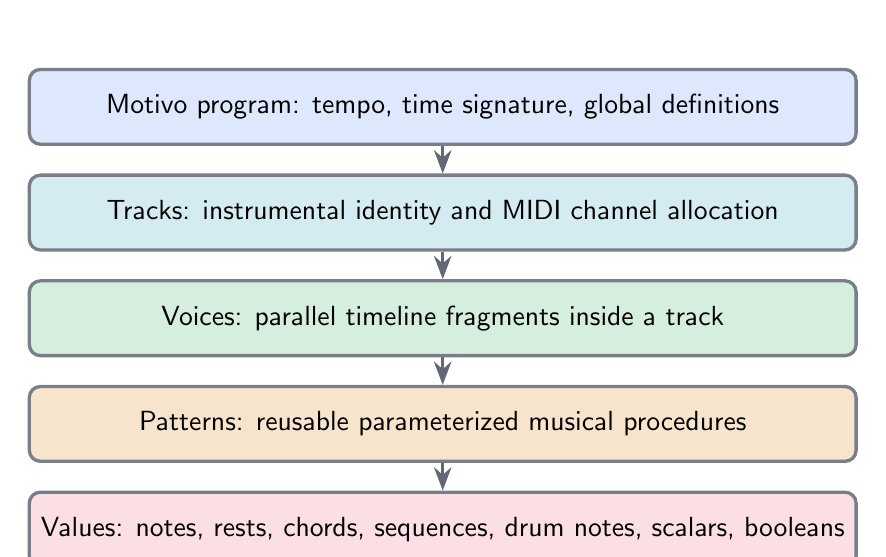
\begin{tikzpicture}[
      level/.style={rounded corners=4pt, draw=motivoInk!60, very thick, minimum width=10.5cm, minimum height=0.95cm,
      align=center, font=\sffamily},
      arrow/.style={-Stealth, very thick, draw=motivoInk!70}
    ]
    \node[level, fill=motivoBlue!15] (program) {Motivo program: tempo, time signature, global definitions};
    \node[level, fill=motivoCyan!18, below=0.35cm of program] (track) {Tracks: instrumental identity and MIDI
    channel allocation};
    \node[level, fill=motivoGreen!18, below=0.35cm of track] (voice) {Voices: parallel timeline fragments
    inside a track};
    \node[level, fill=motivoAmber!20, below=0.35cm of voice] (pattern) {Patterns: reusable parameterized
    musical procedures};
    \node[level, fill=motivoRose!14, below=0.35cm of pattern] (values) {Values: notes, rests, chords,
    sequences, drum notes, scalars, booleans};

    \draw[arrow] (program) -- (track);
    \draw[arrow] (track) -- (voice);
    \draw[arrow] (voice) -- (pattern);
    \draw[arrow] (pattern) -- (values);
  \end{tikzpicture}
  \caption{Motivo's source-level hierarchy.
  The compiler validates this hierarchy before lowering it into timestamped note events.}\label{fig:motivo-hierarchy}
\end{figure}

\section{Source Syntax and Formal Grammar}\label{sec:source-grammar}

Motivo is defined by a formal grammar that ensures syntactic consistency and enables the generation of an
Abstract Syntax Tree (AST).
This grammar is divided into a lexical specification (the scanner) and a context-free grammar (the parser).

\subsection{Lexical Grammar}\label{detail-subsec:lexical-grammar}

The lexical layer tokenizes the raw source text into a stream of symbols.
A notable feature of the lexical grammar is the inclusion of musical literals as first-class tokens.
For example, a note literal is defined by the regular expression \verb|[A-G][#b]?[0-8]|, allowing the scanner to
directly recognize pitches such as \texttt{F\#4} or \texttt{Bb2}.
Keywords are reserved for musical structural elements (\texttt{track}, \texttt{pattern}, \texttt{voice}), temporal
modifiers (\texttt{play}, \texttt{from}, \texttt{rest}), and standard programming constructs (\texttt{let},
\texttt{for}, \texttt{if}).

\subsection{Syntactic Grammar}\label{detail-subsec:syntactic-grammar}

The syntactic grammar follows an EBNF (Extended Backus-Naur Form) structure.
It is designed to enforce the hierarchical relationship between musical components.
The root of a program consists of tempo and time-signature metadata followed by top-level declarations.
Key-signature declarations are not part of the current language and are treated later as future work.

\begin{figure}[htbp]
  \centering
  \begin{lstlisting}[basicstyle=\ttfamily\scriptsize,breaklines=true]
<program>    ::= <header> <top-item>*
<top-item>   ::= <let-stmt> | <pattern-def> | <track-decl>
<track-decl> ::= "track" IDENT? ("using" <inst>)? "{" <track-body> "}"
<track-body> ::= (<stmt> | <pattern-def> | <voice-decl>)*
<pattern>    ::= "pattern" IDENT "(" <params> ")" "{" <stmt-list> "}"
<play-stmt>  ::= "play" <play-target> ";"
<play-target>::= <source> (":" <expr>)? ("from" <expr>)?
  \end{lstlisting}
  \caption{Simplified EBNF representation of the core Motivo grammar.}\label{fig:grammar-ebnf}
\end{figure}

The grammar allows for both braced and unbraced statement bodies in control flow structures, providing a balance between
clarity and brevity.
Crucially, the grammar restricts certain constructs based on their context; for instance, while a \texttt{track} can
contain multiple \texttt{voice} blocks, a \texttt{voice} cannot nest another \texttt{track}, enforcing a one-to-one
mapping between tracks and instrument identities.
The expression sub-grammar supports a full range of arithmetic and logical operators, including a ternary conditional
operator, enabling complex musical logic to be expressed inline.

\section{Musical Primitives and Compositional Constructs}\label{sec:musical-primitives}

To bridge the gap between abstract musical theory and formal computer science, the Motivo language maps
fundamental musical
entities to specific programming constructs.
This mapping ensures that the language remains expressive for musicians while retaining the type safety and structural
clarity of a compiled language.

\subsection{Musical Entities as Data Types}\label{detail-subsec:musical-entities-as-data-types}

The language defines core primitives that serve as the building blocks of a composition.

\noindent \textbf{Notes.} Represented as pitch-class and octave pairs (e.g., \texttt{C4}, \texttt{F\#2}).
These are treated as constant literals with unique numeric identifiers in the underlying MIDI protocol.

\noindent \textbf{Chords.} Modeled as collections of simultaneous notes.
In Motivo, a chord is a single unit of duration, where the temporal span is determined by its constituent notes.

\noindent \textbf{Sequences.} Represented as ordered lists of musical events (notes, chords, or rests).
This structure maps directly to the concept of a musical ``bar'' or ``cell''.

\noindent \textbf{Rests.} Unlike many languages that use a \texttt{sleep} function to pause execution, this
domain-specific language treats a
rest as a durational value.
A rest is a ``silent note'' that occupies space in the timeline, maintaining the structural alignment of the
composition.

\subsection{Compositional Abstractions}\label{detail-subsec:compositional-abstractions}

The hierarchical organization of music is reflected in the language's scoping and container constructs:

\subsubsection{Patterns: The Unit of Reusability}
A \texttt{pattern} is the primary abstraction mechanism in Motivo\@.
Semantically, it is equivalent to a function definition.
It allows a composer to encapsulate a motif and assign it a name.
Patterns can accept parameters, enabling the creation of dynamic musical ideas---such as a drum fill that
varies based on
a boolean flag or a melodic line that accepts a sequence as a template.

\subsubsection{Tracks: Instrumental Identity}
A \texttt{track} serves as the top-level execution context for a specific instrument.
In the compilation process, each track maps to a unique MIDI channel.
This means that independent musical lines (e.g., a piano melody and a bassline) are kept separate and assigned to
distinct sound patches in the final artifact.

\subsubsection{Voices: Horizontal Parallelism}
Within a single track, the \texttt{voice} construct allows for polyphonic composition.
While a track represents a single ``performer'', a voice represents a single ``line of counterpoint''.
Multiple voices can be defined to start at the same time or at different offsets within the same track, allowing for
complex harmonic structures without the need for manual delta-time calculations.
Voices enable the composer to think in terms of horizontal layers rather than just vertical chords.

\section{Imperative Syntax for Algorithmic Variation}\label{sec:syntax-design}

The choice of syntax in a domain-specific language is a critical decision that influences both the learning curve and
the expressiveness of the language.
For Motivo, a C-style imperative syntax was selected for its familiarity and its ability to clearly represent
the deterministic progression of a musical program.

\subsection{Familiarity and Cognitive Load}\label{detail-subsec:familiarity-and-cognitive-load}

By adopting standard programming conventions---such as curly braces for blocks, semicolons for statement
termination, and
parentheses for parameters---Motivo targets a user base that is already familiar with general-purpose languages like C,
C++, or Java.
This choice reduces the cognitive load on the user, allowing them to focus on the musical logic rather than learning a
completely novel syntactical paradigm.
This contrasts with languages like \textit{Tidal}, which rely on deeply nested functional structures that can be opaque
to users without a strong Haskell background.

\subsection{Imperative Flow as a Musical Metaphor}\label{detail-subsec:imperative-flow-as-a-musical-metaphor}

Musical composition is often an imperative process: ``play this, then repeat that, then if a condition is met, change
this''.
Motivo's control flow structures map directly to these compositional needs:

\noindent \textbf{Loops (\texttt{loop}, \texttt{for}):} The \texttt{loop} construct provides a simple mechanism for
repetition (e.g., a constant drum beat).
The C-style \texttt{for} loop enables more complex \textit{algorithmic composition}, where an index variable can
drive musical parameters.
For example, a loop can transpose a motif incrementally by using the iterator value as a pitch offset.

\noindent \textbf{Conditionals (\texttt{if}, \texttt{else}):} These structures allow for \textit{context-aware
composition}.
A phrase might have a different ending depending on whether it is the first or second time it is played, or a track
might include a crash cymbal accent only on the first beat of a section.

\subsection{Algorithmic Variation vs. Static
Definition}\label{detail-subsec:algorithmic-variation-vs.-static-definition}

Traditional MIDI editing is inherently static; a motif is a series of fixed events.
The imperative syntax of Motivo allows motifs to be defined \textit{algorithmically}.
By combining control flow with variables (\texttt{let}), a composer can write code that generates variations of a theme
without manually copying and pasting events.
This methodology reinforces the idea that music is not just a sequence of data points, but a series of logical
instructions that can be computed.
Since the compiler unrolls these instructions at compile-time, the composer enjoys the power of algorithmic generation
without the overhead or latency of a real-time interpreter.

The following compact example shows the intended relationship between imperative notation and musical
structure. The source program contains no MIDI status bytes and no delta-time calculations. It expresses a
bar-level rule, and the compiler expands that rule into concrete events.

\begin{lstlisting}[language=Motivo, caption={A compact Motivo drum pattern.}, label={lst:motivo-groove}]
tempo 128;
signature 4/4;

track percussion using drums {
    pattern bar() {
        for (let i = 0; i < 16; i = i + 1) {
            play hihat from i;
            if (i % 8 == 0) { play kick from i; }
            if (i % 8 == 4) { play snare from i; }
        }
    }

    loop (500) { play bar(); }
}
\end{lstlisting}

\section{Compiler Pipeline and Implementation Foundations}\label{sec:compiler-pipeline}

The architecture of Motivo compiler is organized as a multi-pass pipeline.
Each stage of the pipeline transforms the representation of the musical program, moving from abstract textual intent to
a concrete binary artifact.
By decoupling these stages, the compiler ensures that errors are caught early and that the musical structure is fully
resolved before generation.

\subsection{Information Flow and Artifacts}\label{detail-subsec:information-flow-and-artifacts}

The flow of data through the compiler is illustrated in Figure~\ref{fig:compiler-pipeline}.
Each box represents a discrete processing stage, and the annotated arrows describe the intermediate artifacts passed
between them.

\subsection{Transformation Stages}\label{detail-subsec:transformation-stages}

The transformation process is organized into four stages.

\noindent \textbf{Text to Tree (Frontend).} The raw source text is parsed into an \textit{Abstract Syntax Tree} (AST).
This artifact captures the logical hierarchy of the composition (e.g., nested patterns and tracks) but contains no
musical or temporal resolution.

\noindent \textbf{Tree to Annotated Tree (Semantic Analysis).} The compiler performs symbol resolution and
type inference.
The resulting \textit{Annotated AST} links every identifier to its definition and ensures that all operations are
musically valid.

\noindent \textbf{Tree to Timeline (Lowering).} The hierarchical AST is ``unrolled'' into a flat \textit{Intermediate
Representation} (IR).
This is the most significant transformation, where recursive pattern calls and loops are replaced by a sorted list
of concrete \texttt{NoteEvents} with absolute timestamps.

\noindent \textbf{Timeline to Binary (Backend).} Finally, the IR is serialized.
The backend converts the absolute timestamps into the delta-times required by the MIDI standard and writes the
structured binary stream to disk.

\begin{figure}[htbp]
  \centering
  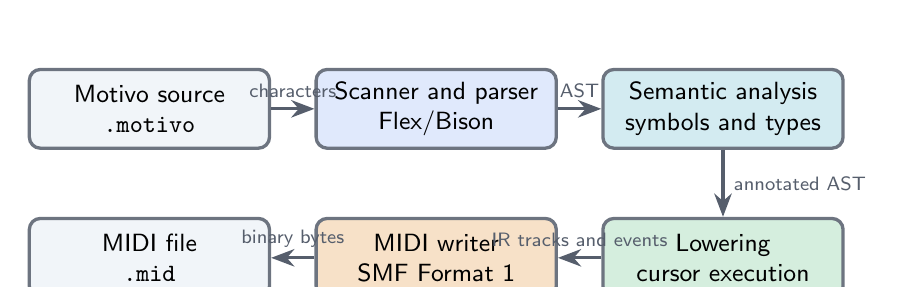
\begin{tikzpicture}[
      stage/.style={rounded corners=4pt, draw=motivoInk!65, very thick, minimum width=3.05cm, minimum height=1.0cm,
      align=center, font=\small\sffamily},
      artifact/.style={font=\scriptsize\sffamily, text=motivoInk!75, align=center},
      arrow/.style={-Stealth, very thick, draw=motivoInk!75}
    ]
    \node[stage, fill=motivoSoft] (src) {Motivo source\\\texttt{.motivo}};
    \node[stage, fill=motivoBlue!14, right=0.55cm of src] (parse) {Scanner and parser\\Flex/Bison};
    \node[stage, fill=motivoCyan!18, right=0.55cm of parse] (sem) {Semantic analysis\\symbols and types};
    \node[stage, fill=motivoGreen!18, below=0.85cm of sem] (low) {Lowering\\cursor execution};
    \node[stage, fill=motivoAmber!22, left=0.55cm of low] (midi) {MIDI writer\\SMF Format 1};
    \node[stage, fill=motivoSoft, left=0.55cm of midi] (out) {MIDI file\\\texttt{.mid}};

    \draw[arrow] (src) -- node[artifact, above] {characters} (parse);
    \draw[arrow] (parse) -- node[artifact, above] {AST} (sem);
    \draw[arrow] (sem) -- node[artifact, right] {annotated AST} (low);
    \draw[arrow] (low) -- node[artifact, above] {IR tracks and events} (midi);
    \draw[arrow] (midi) -- node[artifact, above] {binary bytes} (out);
  \end{tikzpicture}
  \caption{Motivo compiler data flow from source text to Standard MIDI File.}\label{fig:compiler-pipeline}
\end{figure}

\subsection{Technical Foundations and Build Structure}\label{subsec:implementation-foundations}

The implementation of Motivo compiler is a critical engineering effort that balances high-level musical expressiveness
with low-level binary precision.
The discussion details the selection of the technology stack and the structural organization of the project, providing a
rationale for the architectural decisions that support the thesis's goals.

\subsection{Language Choice: Modern C++ (C++23)}\label{detail-subsec:language-choice:-modern-c++-(c++23)}

The compiler is written in modern C++, specifically targeting the C++23 standard.
While higher-level languages such as Python or JavaScript are commonly used for domain-specific language
development, C++ was selected for
three primary reasons:

\noindent \textbf{Deterministic Performance.} Musical temporal resolution requires high precision.
By using C++, the compiler can perform recursive unrolling and temporal math with minimal overhead, achieving the
fast local compilation times necessary for real-time feedback in the playground.

\noindent \textbf{Robust Type System.} Modern C++ provides a wealth of tools for building type-safe compilers.
Features such as \texttt{std::variant} and \texttt{std::optional} allow for a functional programming style that is
ideally suited for processing tree-like structures (ASTs).

\noindent \textbf{Binary Serialization.} Since the final build target is a low-level MIDI binary file, C++'s native
support for
bitwise operations and big-endian serialization makes it a practical choice for implementing the backend.

\subsubsection{C++23 Features Used in the Architecture}

The codebase leverages several advanced features to simplify compiler logic:

\noindent \textbf{\texttt{std::variant} as a Sum Type:} Every AST node and IR value is represented as a variant.
This allows the compiler to treat different musical constructs (e.g., a Note vs a Loop) as a single type while
enforcing exhaustive handling during traversal via \texttt{std::visit}.

\noindent \textbf{Value-Oriented Memory Management.} By combining \texttt{std::variant} with
\texttt{std::unique\_ptr}, the
compiler avoids the ``Object Soup'' anti-pattern.
Nodes are value-like, and recursion is handled via smart pointers that support explicit ownership and reduced
leak risk without the
non-deterministic latency of a garbage collector.

\noindent \textbf{Standard Ranges and Views.} Used extensively in the backend and lowering passes to sort musical events
and filter diagnostic logs efficiently.

\subsection{Modular Build Infrastructure (CMake)}\label{detail-subsec:modular-build-infrastructure-(cmake)}

To ensure scalability and maintainability, the project is structured as a modular hierarchy managed by
CMake~\cite{CMake_2026}.
The source code is partitioned into discrete components, each with its own responsibilities and boundaries.

\subsubsection{Library Decomposition}

The compiler logic is distributed across static libraries with separate responsibilities.

\noindent \textbf{\texttt{motivo\_common}:} The foundational library containing the core musical enums (\texttt{Pitch},
\texttt{Accidental}), the \texttt{Note} structure, and the \texttt{DiagnosticsEngine}.
It is linked by every other module.

\noindent \textbf{\texttt{motivo\_frontend}:} Wraps the Flex-generated scanner and Bison-generated parser.
It depends on \texttt{motivo\_common} for location tracking and note literals.

\noindent \textbf{\texttt{motivo\_semantic}:} Contains the \texttt{Traversal} engine and symbol table logic.
It takes a raw AST and produces an \texttt{AnalysisResult}.

\noindent \textbf{\texttt{motivo\_lowerer}:} The unrolling engine.
It transforms an \texttt{AnalysisResult} into a flat list of \texttt{NoteEvent} objects.

\noindent \textbf{\texttt{motivo\_backend}:} The MIDI serialization module.
It handles the binary translation of the linear event stream.

\subsubsection{Directory Organization and Public API}

The project separates public interfaces from private implementation files.

\noindent \textbf{\texttt{include/motivo/}:} Contains only the public headers (e.g., \texttt{compiler.hpp}).
This defines the interface for external consumers, such as the CLI wrapper or the playground backend.

\noindent \textbf{\texttt{src/motivo/}:} Contains the private implementation details, including the recursive
visitors and
generated Flex/Bison sources.

This separation ensures that the internal complexity of the compiler pipeline is hidden behind a simple, high-level
API\@.
The top-level \texttt{motivo::compile} function serves as the entry point, orchestrating the sequential flow
of characters
to tree, tree to timeline, and timeline to MIDI\@.

\section{Frontend and Abstract Syntax Tree Construction}\label{sec:implementation-frontend}

The frontend is the gatekeeper of the compiler, responsible for validating the syntactic structure of the user's input
and building a logical model of the composition.
This phase is implemented using a classic scanner-parser architecture.

\subsection{Lexical Analysis: Identifying Musical
Literals}\label{detail-subsec:lexical-analysis:-identifying-musical-literals}

The scanner, implemented in \texttt{scanner.l} using Flex, transforms the source code's character stream into a sequence
of tokens~\cite{Flex_2026}.
The most technically significant challenge in the lexical pass was the requirement for first-class musical literals.

\subsubsection{Pitch-Class and Note Recognition}

Unlike conventional languages that treat musical data as strings or numbers, Motivo treats a pitch like
\texttt{F\#4} as
a primitive constant.
The scanner utilizes a specialized regular expression to recognize these patterns:
\begin{lstlisting}[caption={Flex regular expression for note literal recognition.},label={detail-lst:lstlisting}]
pitch        [A-G]
accidental   [#b]
octave       [0-8]
note_lit     {pitch}{accidental}?{octave}
\end{lstlisting}

When this pattern is matched, the scanner does not simply return a token; it invokes
\texttt{parse\_note\_literal}, which
decomposes the string into a \texttt{music::Note} structure (containing the pitch enum, accidental enum, and octave
integer).
This means that the ``musicality'' of the code is validated at the very first byte of processing.

\subsubsection{Keyword and Symbol Disambiguation}

The scanner also manages a set of reserved keywords that define the structural identity of the language.
Keywords such as \texttt{track}, \texttt{pattern}, and \texttt{voice} transition the parser into different scoping
states.
Additionally, the scanner implements ``Longest-Match'' logic to ensure that identifiers starting with keyword names
(e.g., a variable named \texttt{loop\_count}) are not incorrectly tokenized as keywords.

\subsection{Syntactic Analysis: Building the Hierarchy}\label{detail-subsec:syntactic-analysis:-building-the-hierarchy}

The parser, implemented in \texttt{parser.y} using Bison, is a LALR parser with one-token
lookahead~\cite{GNU_Bison_2026}.
Its primary role is to enforce the context-free grammar and construct the Abstract Syntax Tree (AST).

\subsubsection{AST Node Architecture and Sum-Types}

The AST is designed as a set of recursive structures defined in the \texttt{motivo::ast} namespace.
To achieve type safety, the implementation utilizes the ``Sum-Type'' pattern via
\texttt{std::variant}.

\paragraph{Declaration and Definition Nodes}
The top-level structure of the AST is represented by definitions that manage scoping and vertical layering:

\noindent \textbf{\texttt{TrackDefinition}:} Holds an optional name, an optional instrument, and a body of
\texttt{TrackItem} nodes.
A \texttt{TrackItem} is a variant that can hold a statement, a local pattern, or a voice.

\noindent \textbf{\texttt{PatternDefinition}:} A node that captures the signature of a musical function, including its
name, parameter list, and a block of statements.

\noindent \textbf{\texttt{VoiceDefinition}:} Represents horizontal parallelism.
It stores an optional \texttt{from} expression and a body of statements and local patterns.

\paragraph{Statement and Expression Polymorphism}
The leaf nodes of the tree are divided into statements (actions) and expressions (values):

\noindent \textbf{\texttt{StatementKind}:} Contains nodes like \texttt{AssignStatement}, \texttt{ForStatement},
\texttt{IfStatement}, \texttt{LetStatement}, \texttt{LoopStatement}, and \texttt{PlayStatement}.

\noindent \textbf{\texttt{ExpressionKind}:} A variant containing literals (\texttt{Int}, \texttt{Float}, \texttt{Bool},
\texttt{Note}, \texttt{Rest}), identifiers for variable lookup, unary/binary operations, and complex musical
structures like \texttt{SequenceExpression} and \texttt{ChordExpression}.

\subsubsection{Recursive Node Ownership}

To maintain the tree hierarchy, recursive nodes (e.g., the condition of an \texttt{if} statement) are wrapped in
\texttt{std::unique\_ptr}.
This design choice was made to ensure that the AST is a true tree structure in memory, while the use of
\texttt{std::variant} at every level ensures that the compiler can traverse the tree using ``Pattern Matching'' in the
subsequent semantic and lowering passes.
This combination of value-oriented variants and pointer-based recursion provides a robust foundation for the multi-pass
architecture.

\section{Semantic Analysis and Validation}\label{sec:semantic-rules}

After the frontend produces a syntactically correct Abstract Syntax Tree, the compiler enters the \textit{Semantic
Analysis} phase.
This stage is responsible for ensuring that the program is logically and musically sound.
It performs three primary tasks: identifier resolution (scoping), type inference, and musical constraint validation.

\subsection{Architectural Pattern: The Recursive
Visitor}\label{detail-subsec:architectural-pattern:-the-recursive-visitor}

The semantic analyzer is implemented in the compiler's semantic traversal class.
Because the AST uses \texttt{std::variant} for statement and expression polymorphism, the analyzer relies on a visitor
pattern implemented with \texttt{std::visit} and a small overloaded-helper template.
This allows the compiler to dispatch logic cleanly based on the concrete type of the AST node without relying on dynamic
casting or virtual method tables.

The traversal process follows a precise lifecycle designed to support the hierarchical nature of Motivo\@:

\noindent \textbf{Global Collection.} The analyzer first iterates over all top-level global items.
It extracts all \texttt{PatternDefinition} nodes and registers them in the global scope.
This ``pre-pass'' enables forward referencing, allowing a track at the beginning of a file to call a pattern defined
at the end.

\noindent \textbf{Track and Voice Entry.} For each \texttt{TrackDefinition}, the analyzer enters a new lexical scope.
It performs a similar pre-pass to collect track-local patterns before traversing the body statements.
The same logic applies when visiting a \texttt{VoiceDefinition}.

\noindent \textbf{Recursive Resolution.} Expressions are evaluated bottom-up.
A binary expression node, for instance, will recursively visit its left and right children, infer their types,
validate their compatibility, and then determine its own resulting type.

\subsection{Symbol Table and Scope Management}\label{detail-subsec:symbol-table-and-scope-management}

Scoping is managed by the \texttt{SymbolTable} and \texttt{ScopeStack} classes.
The \texttt{SymbolTable} maintains the actual symbol data, while the \texttt{ScopeStack} manages the hierarchical
environment during the AST traversal.

\subsubsection{Hierarchical Scoping Rules}

The \texttt{ScopeStack} maintains a stack of \texttt{ScopeId} references pointing to the \texttt{SymbolTable}.
Scopes are pushed and popped as the visitor enters and exits structural nodes (Global, Track, Voice, Pattern, and
Control Flow Blocks).
The implementation enforces strict visibility rules:

\noindent \textbf{Lookup.} When an \texttt{IdentifierExpression} is encountered, the \texttt{ScopeStack} performs a
reverse search from the current scope up to the global scope.
If the identifier is found, its unique \texttt{SymbolId} and inferred \texttt{Type} are retrieved.

\noindent \textbf{Symbol Metadata.} Every registered symbol stores its \texttt{SymbolKind} (Variable,
  Parameter, Pattern,
Track, or Voice), its declared \texttt{Location} in the source file, and a raw pointer back to its declaration node
in the AST\@.

\subsubsection{AST Annotation}

To separate analysis from execution, the semantic pass does not mutate the original AST structure.
Instead, it populates an \texttt{Annotations} object.
Upon successful resolution of an identifier, the \texttt{Annotations} object maps the memory address of the
\texttt{IdentifierExpression} to its resolved \texttt{SymbolId}.
Similarly, every evaluated expression is mapped to its inferred \texttt{Type}.
This metadata ensures that the subsequent ``Lowering'' pass does not need to perform expensive string lookups or type
checks; it simply retrieves the cached resolution data.

\subsection{Formal Type Rules and Constraints}\label{detail-subsec:formal-type-rules-and-constraints}

The type system acts as the ``Musical Guardrail'' of the compiler, implemented in the \texttt{type\_rules.cpp} module.

\subsubsection{Type Categories}
The analyzer categorizes types into the \texttt{TypeKind} enumeration:

\noindent \textbf{Scalars.} \texttt{Int}, \texttt{Double}, \texttt{Bool}.
These are utilized for mathematical operations, loop counts, and conditional logic.

\noindent \textbf{Musical Primitives.} \texttt{Note}, \texttt{Rest}, \texttt{Chord}, \texttt{Sequence}, \texttt{Drum}.
These represent the playable entities that occupy space on the timeline.

\noindent \textbf{Utility Types.} \texttt{Unknown} (used during error recovery) and \texttt{Void} (for statements that
produce no value).

\subsubsection{Constraint Validation Logic}
The analyzer enforces critical invariants through specific validator methods within the \texttt{Traversal} class:

\noindent \textbf{\texttt{validate\_binary\_operands}:} Ensures that arithmetic operators (\texttt{+}, \texttt{-},
\texttt{*}, \texttt{/}, \texttt{\%}) are strictly applied to numeric scalars (\texttt{Int} or \texttt{Double}).
For example, attempting to add two sequences (\texttt{[C4] + [D4]}) will trigger a semantic error, as musical
concatenation is handled differently than arithmetic addition.

\noindent \textbf{\texttt{validate\_play\_target}:} This method verifies that the target of a \texttt{play}
statement resolves to a valid musical primitive.
If a composer mistakenly writes \texttt{play (i < 5);}, the analyzer intercepts the error because the target
evaluates to a \texttt{Bool}.

\noindent \textbf{\texttt{validate\_pattern\_instantiation}:} When a \texttt{PatternCallExpression} is visited,
the analyzer
performs a virtual instantiation.
It creates a temporary scope, binds the parameter names to the types of the arguments provided at the call site, and
recursively visits the pattern's body block.
This allows the compiler to catch type errors \textit{inside} a pattern that only manifest when it is invoked with
specific argument types, ensuring deep semantic validation.

\section{Timeline Semantics and Cursor-Based Time}\label{sec:temporal-model}

A central challenge in music programming is the representation of time.
While physical time is continuous, musical time is often perceived as a series of discrete units (beats, bars,
subdivisions).
Motivo uses a deterministic \textit{cursor model} to manage temporal placement, providing a balance
between sequential flow and absolute positioning.

\subsection{The Virtual Playhead}\label{detail-subsec:the-virtual-playhead}

The core of the temporal logic is a virtual ``playhead'' or \textit{cursor}.
As the compiler traverses the musical statements within a track or voice, it maintains an internal state representing
the current absolute beat position.
Every musical command interacts with this cursor in one of two ways:

\noindent \textbf{Relative Advancement.} Standard \texttt{play} and \texttt{rest} statements are relative to the current
cursor position.
When a note is played, it is placed at the current cursor value, and the cursor is subsequently advanced by the
duration of that note.
This model allows for natural, sequential composition that mimics the act of writing on a staff.

\noindent \textbf{Absolute Offsets.} The \texttt{from} keyword allows for non-destructive positioning.
A statement such as \texttt{play A4 from 16;} places a note at the 16th beat regardless of the current cursor
position.
Crucially, this operation does not advance the main cursor, allowing the composer to ``jump'' back and forth across
the timeline to layer multiple events without losing the primary sequential flow.

\subsection{Parallelism and Temporal Isolation}\label{detail-subsec:parallelism-and-temporal-isolation}

The cursor model is also applied to parallel structures.
When a \texttt{voice} is defined within a \texttt{track}, it inherits a copy of the parent track's current cursor
position.
However, advancements within the voice are isolated; they do not affect the cursor of the parent track or of sibling
voices.
This allows for the creation of independent rhythmic layers that are synchronized at their start point but proceed at
their own pace.

\subsection{Deterministic Time Resolution}\label{detail-subsec:deterministic-time-resolution}

By using floating-point arithmetic for the internal cursor, the language supports arbitrary rhythmic subdivisions
(e.g., triplets, dotted notes, or complex swing rhythms).
Unlike interpreted systems that may suffer from timing drift or ``jitter'' due to CPU scheduling, the compiled nature of
Motivo calculates every event before writing the output file, so event placement is resolved before playback.
Time is resolved entirely during the ``Lowering'' phase of the compiler, transforming the hierarchical code into a flat,
sorted timeline of events.
This methodology keeps musical placement deterministic within the current mapping.

\begin{figure}[htbp]
  \centering
  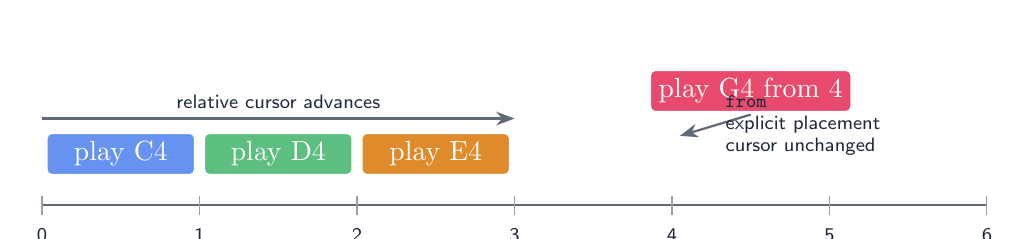
\begin{tikzpicture}[
      beat/.style={font=\scriptsize\sffamily, text=motivoInk},
      note/.style={rounded corners=2pt, minimum height=0.42cm, draw=white, very thick},
      arrow/.style={-Stealth, thick, draw=motivoInk!70}
    ]
    \draw[thick, draw=motivoInk!70] (0,0) -- (12,0);
    \foreach \x/\b in {0/0,2/1,4/2,6/3,8/4,10/5,12/6} {
      \draw[draw=motivoInk!45] (\x,0.12) -- (\x,-0.12);
      \node[beat, below=0.18cm] at (\x,0) {\b};
    }

    \node[note, fill=motivoBlue!70, minimum width=1.9cm] at (1,0.65) {\textcolor{white}{play C4}};
    \node[note, fill=motivoGreen!70, minimum width=1.9cm] at (3,0.65) {\textcolor{white}{play D4}};
    \node[note, fill=motivoAmber!85, minimum width=1.9cm] at (5,0.65) {\textcolor{white}{play E4}};
    \node[note, fill=motivoRose!80, minimum width=1.9cm] at (9,1.45) {\textcolor{white}{play G4 from 4}};

    \draw[arrow] (0,1.1) -- node[beat, above] {relative cursor advances} (6,1.1);
    \draw[arrow] (9,1.15) -- node[beat, right, align=left] {\texttt{from}\\explicit placement\\cursor
    unchanged} (8.1,0.88);
  \end{tikzpicture}
  \caption{Cursor-based temporal placement.
    Sequential statements advance the cursor, while \texttt{from} positions an event on the timeline
  explicitly.}\label{fig:cursor-model}
\end{figure}

\section{Compilation Strategy: Deterministic Unrolling}\label{sec:compilation-strategy}

Motivo is designed as a fully compiled language, distinguishing it from interpreted musical environments.
This design choice is driven by the mandate for a \textit{zero-runtime architecture}, where all musical and logical
structures are resolved before any sound is produced or any output file is written.

\subsection{The Zero-Runtime Mandate}\label{detail-subsec:the-zero-runtime-mandate}

In a zero-runtime system, the complexity of the composition is handled entirely by the compiler.
This means that features such as nested loops, conditional branching, and recursive pattern calls do not exist in the
output artifact.
Instead, the compiler performs a process of \textit{deterministic unrolling}.
Every loop is expanded into its constituent iterations, every conditional branch is evaluated and resolved, and every
pattern call is inlined.

The result of this process is an Intermediate Representation (IR) that consists of a flat, linear list of atomic musical
events.
This architecture provides several benefits:

\noindent \textbf{High Performance.} The output artifact is extremely lightweight, as all logical overhead has been
removed.

\noindent \textbf{Offline Validation.} Semantic errors---such as variable shadowing, type mismatches, or
invalid rhythmic
math---are caught during the compilation phase, providing immediate feedback to the composer.

\noindent \textbf{Portability.} The resulting IR can be easily serialized into formats beyond MIDI in future extensions
without requiring a specialized interpreter to read it.

\subsection{Temporal Reconstruction of Patterns}\label{detail-subsec:temporal-reconstruction-of-patterns}

A unique aspect of the compilation strategy is how the temporal span of a pattern is reconstructed.
When a pattern is called, the compiler does not just emit the notes within it; it calculates the total duration occupied
by the pattern, including internal gaps and trailing rests.
This is achieved by capturing the state of the internal cursor before and after the pattern's body is unrolled.
The difference between these two points defines the pattern's ``footprint'' on the timeline, allowing the pattern to be
treated as a single, opaque musical unit by the caller.

\subsection{Static Verification of Compositional Logic}\label{detail-subsec:static-verification-of-compositional-logic}

Because the language is compiled, it can enforce constraints that would be difficult to manage in an interpreted system.
The semantic analysis pass verifies that the composition adheres to the physical limits of the target protocol (e.g.,
ensuring notes are within the MIDI pitch range of 0--127) and that the structural hierarchy is valid (e.g., preventing a
\texttt{track} from being defined inside a \texttt{pattern}).
This validation is intended to ensure that the final MIDI artifact is not only syntactically correct but also musically
meaningful and interoperable with MIDI-aware tools.

\begin{figure}[htbp]
  \centering
  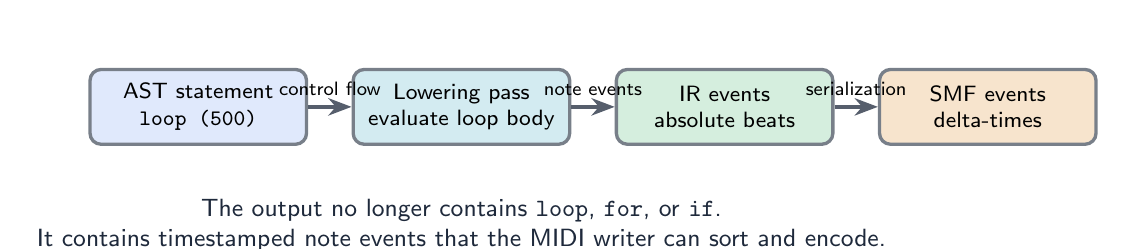
\begin{tikzpicture}[
      box/.style={rounded corners=4pt, draw=motivoInk!60, very thick, minimum width=2.75cm, minimum height=0.95cm,
      align=center, font=\footnotesize\sffamily},
      arrow/.style={-Stealth, very thick, draw=motivoInk!75}
    ]
    \node[box, fill=motivoBlue!14] (ast) {AST statement\\\texttt{loop (500)}};
    \node[box, fill=motivoCyan!18, right=0.55cm of ast] (exec) {Lowering pass\\evaluate loop body};
    \node[box, fill=motivoGreen!18, right=0.55cm of exec] (ir) {IR events\\absolute beats};
    \node[box, fill=motivoAmber!20, right=0.55cm of ir] (smf) {SMF events\\delta-times};

    \draw[arrow] (ast) -- node[above, font=\scriptsize\sffamily] {control flow} (exec);
    \draw[arrow] (exec) -- node[above, font=\scriptsize\sffamily] {note events} (ir);
    \draw[arrow] (ir) -- node[above, font=\scriptsize\sffamily] {serialization} (smf);

    \node[below=0.55cm of exec, align=center, font=\small\sffamily, text=motivoInk] {
      The output no longer contains \texttt{loop}, \texttt{for}, or \texttt{if}.\\
      It contains timestamped note events that the MIDI writer can sort and encode.
    };
  \end{tikzpicture}
  \caption{Lowering removes source-level control flow by expanding it into concrete musical
  events.}\label{fig:ast-to-ir}
\end{figure}

\section{Lowering Engine and Intermediate Representation}\label{sec:lowering-ir}

The \textit{Lowering Engine} is the most sophisticated component of the compiler.
It performs the transformation from the hierarchical, logically structured Annotated AST into a flat, chronologically
sorted list of events known as the Intermediate Representation (IR).
This process ``unrolls'' the recursive structure of the music and resolves all temporal logic into absolute beat
offsets, effectively stripping away all programming control flow.

\subsection{The Intermediate Representation (IR)}\label{detail-subsec:the-intermediate-representation-(ir)}

The output of the lowering engine is an \texttt{ir::Program} object.
This artifact represents the physical timeline of the composition.
Its primary building block is the \texttt{NoteEvent} structure:

\begin{lstlisting}[language=C++, caption={Structure of an atomic IR event.},label={detail-lst:lstlisting2}]
struct NoteEvent {
    int midi_note;          // Numeric pitch (0-127)
    double start_beat;      // Absolute position from track start
    double duration_beats;  // Temporal span in beats
    int velocity;           // MIDI intensity (default 100)
};
\end{lstlisting}

An important architectural detail is that the IR is entirely agnostic of the language's original control flow.
Whether a note was generated by a static \texttt{play} command, a \texttt{for} loop iteration, or a recursive
\texttt{pattern} call, it is represented in the IR as a simple, independent data point.

\subsection{Stateful Unrolling and Cursor Management}\label{detail-subsec:stateful-unrolling-and-cursor-management}

The unrolling engine is managed by the \texttt{LowererContext} class.
Unlike the semantic analyzer, which checks static types, the lowerer acts almost as an interpreter, executing the logic
and managing actual runtime values.
It maintains a ``cursor'' (a \texttt{double} passed by reference) tracking the current playhead position in beats.

The \texttt{lower\_statement} function utilizes \texttt{std::visit} to dispatch logic based on the statement kind:

\noindent \textbf{\texttt{PlayStatement}:} The lowerer evaluates the play target.
It determines the note duration (using the default, or overriding it if the \texttt{:} operator is present).
The start beat is set to the current cursor value, and the event is emitted.
Finally, the cursor is advanced by the duration.
If the \texttt{from} keyword is used, the start beat is overridden by the evaluated offset, and the cursor is
\textit{not} advanced.

\noindent \textbf{\texttt{LoopStatement} and \texttt{ForStatement}:} The engine evaluates the iteration count or
condition, then enters a loop in C++, recursively calling \texttt{lower\_block} for the body.
Because the \texttt{cursor} reference is passed down, the temporal state is naturally preserved across iterations,
placing notes end-to-end.

\noindent \textbf{\texttt{IfStatement}:} The lowerer evaluates the boolean condition into a concrete \texttt{true} or
\texttt{false}.
Only the matching branch is traversed, effectively performing ``compile-time pruning''.

\subsection{Dynamic Expression Evaluation}\label{detail-subsec:dynamic-expression-evaluation}

During the lowering phase, expressions are resolved into concrete values represented by the \texttt{ir::Value} variant.
These values can be scalars (\texttt{int}, \texttt{double}, \texttt{bool}) or musical structures (\texttt{NoteValue},
\texttt{RestValue}, \texttt{SequenceValue}, \texttt{ChordValue}).

The \texttt{LowererContext} maintains a \textit{Dynamic Scope Stack}: a vector of hash maps from identifier names to
\texttt{ir::Value} entries.
When a \texttt{let} or assignment statement is encountered, the evaluated \texttt{ir::Value} is bound to the identifier.
This allows for dynamic algorithmic generation, where loop indices or accumulator variables can be used as multipliers
for note durations or offsets.

\subsection{Value Flattening and Complex Structures}\label{detail-subsec:value-flattening-and-complex-structures}

A significant challenge in the lowering engine is the conversion of complex musical types into atomic
\texttt{NoteEvent}s.
This is handled by the \texttt{ValueFlattener} module.

\subsubsection{Flattening Chords}
When a \texttt{ChordValue} is encountered, the flattener iterates over all its constituent notes and emits them using
the \textit{same} \texttt{start\_beat}.
The main lowering routine then advances the track's cursor by the \textit{maximum} duration found among the chord's
members, ensuring the next musical statement begins only after the entire chord has finished sounding.

\subsubsection{Pattern Temporal Reconstruction}
The most technically complex feature of the lowerer is how it preserves the ``temporal integrity'' of patterns.
When a \texttt{PatternCallExpression} is evaluated:

\noindent The lowerer snapshots the current cursor position: \texttt{start\_time = cursor}.

\noindent It pushes a new variable scope, binds the arguments to the parameter names, and unrolls the pattern's body.

\noindent It captures the final cursor state: \texttt{end\_time = cursor}.

\noindent It calculates the total temporal span as the difference between \texttt{end\_time} and \texttt{start\_time}.

To ensure that internal gaps and trailing rests within the pattern are respected, the lowerer rebuilds a
\texttt{SequenceValue} that intersperses the emitted notes with \texttt{RestValue} items matching the exact temporal
gaps.
This reconstructed value is then returned to the caller, allowing the pattern to be treated as a single, opaque rhythmic
block.

\subsection{Voice Parallelism and Cursor Isolation}\label{detail-subsec:voice-parallelism-and-cursor-isolation}

Parallel melodic lines are managed through the \texttt{voice} construct.
To implement parallelism without shared state conflicts or manual timing math, the lowerer uses
\textit{Cursor Isolation}:

\noindent Upon entering a \texttt{VoiceDefinition}, the lowerer captures the current outer cursor value.

\noindent It creates a local \textit{copy} called \texttt{voice\_cursor}.
If the voice specifies a \texttt{from} expression, the \texttt{voice\_cursor} is initialized to that value instead.

\noindent All statements unrolled within the voice modify only the \texttt{voice\_cursor}.

\noindent The generated \texttt{NoteEvent}s are appended to the track's master list, but upon exiting the
voice block, the
\texttt{outer\_cursor} is completely unmodified.

This isolation keeps the parent track and sibling voices aligned according to the compiler cursor model at
their starting beats, without requiring the author to calculate the intervening offsets manually.

\section{MIDI Domain Logic and Backend Serialization}\label{sec:midi-backend-design}

A primary objective of the implementation is to bridge the gap between high-level musical notation and the low-level
binary encoding required by the MIDI standard.
This section details the mathematical formulas and mapping strategies implemented in the
\texttt{motivo\_music} module to
ensure that the compiler's output is musically accurate.

\subsection{Note to MIDI Pitch Mapping}\label{detail-subsec:note-to-midi-pitch-mapping}

Motivo allows composers to specify pitches using traditional letter names from A to G, accidentals (\#, b), and
octave numbers
(0--8).
The compiler converts these literals into a single numeric byte (0--127) using a deterministic formula.

The implementation defines the \texttt{music::Note} structure as a combination of three fields:

\noindent \textbf{\texttt{Pitch} enum:} Stores the semitone offset within an octave (\texttt{C=0}, \texttt{D=2},
\texttt{E=4}, \texttt{F=5}, \texttt{G=7}, \texttt{A=9}, \texttt{B=11}).

\noindent \textbf{\texttt{Accidental} enum:} Stores a numeric signed offset (\texttt{Flat=-1}, \texttt{Natural=0},
\texttt{Sharp=1}).

\noindent \textbf{\texttt{Octave} integer:} Stores the numeric octave.

The mapping formula used in the \texttt{Note::midi\_number} function is:
\begin{equation}
  P = 12 \times (O + 1) + V_p + V_a\label{eq:midi-pitch-detail}
\end{equation}
Where $P$ is the final MIDI pitch, $O$ is the octave, $V_p$ is the pitch-class value, and $V_a$ is the accidental value.
The constant offset of \textbf{+1} follows the convention used by the compiler and its tests, where \texttt{C4} maps to
MIDI note 60 and \texttt{A4} maps to 69.
By centralizing this calculation at the library level, the compiler ensures that all musical logic throughout the
pipeline is consistent.

\subsection{Instrument and Drum Mapping}\label{detail-subsec:instrument-and-drum-mapping}

The language's \texttt{using} keyword allows the composer to specify the instrumental identity of a track.
This intent is mapped directly to the General MIDI (GM) Level 1 specification.

The implementation utilizes two primary mapping strategies:

\noindent \textbf{Melodic Instruments.} Standard instruments are mapped to their GM program numbers.
For example, \texttt{Piano} maps to 1, \texttt{Guitar} to 24, \texttt{Bass} to 32, and \texttt{Violin} to 40.
These mappings are stored in the \texttt{music::Instrument} enum.
During backend serialization, they are emitted as \textit{Program Change} events on standard MIDI channels (0--8,
11--15).

\noindent \textbf{Percussion Logic.} Unlike melodic tracks, the MIDI standard rigidly reserves \textbf{Channel 10}
specifically for unpitched percussion.
If a track is defined as \texttt{using drums}, the backend automatically routes all its events to Channel 10 and
skips emitting a Program Change event.
Furthermore, individual drum literals in Motivo are mapped to specific GM ``Note-On'' pitches as defined by the
standard drum map:

\noindent \texttt{Kick} $\rightarrow$ 36

\noindent \texttt{Snare} $\rightarrow$ 38

\noindent \texttt{Hihat} $\rightarrow$ 42

\noindent \texttt{Crash} $\rightarrow$ 49

\noindent \texttt{Ride} $\rightarrow$ 51

This explicit mapping aligns drum output with the General MIDI percussion convention in tools that follow that standard.

\begin{table}[htbp]
  \centering
  \renewcommand{\arraystretch}{1.3}
  \begin{tabularx}{\textwidth}{>{\raggedright\arraybackslash}p{3.4cm}X}
    \toprule
    \textbf{Motivo concept} & \textbf{Backend representation} \\
    \midrule
    Tempo declaration & MIDI tempo meta event in track 0. \\
    Time signature declaration & MIDI time-signature meta event in track 0. \\
    Track using piano, guitar, bass, or violin & Separate MIDI track with a Program Change event. \\
    Track using drums & Separate MIDI track routed to the percussion channel. \\
    Note event & Note-On and Note-Off messages with tick positions derived from beats. \\
    Rest & Cursor advancement without emitted note messages. \\
    Chord & Several note events with the same start beat. \\
    Sequence & Sequential flattening of notes, chords, and rests. \\
    \bottomrule
  \end{tabularx}
  \caption{Mapping from Motivo source concepts to MIDI backend artifacts.}\label{tab:motivo-midi-mapping}
\end{table}

\subsection{Binary Serialization of Standard MIDI Files}\label{subsec:midi-binary-serialization}

The final stage of the compilation pipeline translates the flat list of linear \texttt{NoteEvent}s (the IR) into a
Standard MIDI File (SMF) Format 1 binary artifact.
This process requires careful management of binary structures, delta-time calculations, and variable-length encodings.

\subsection{SMF Format 1 Structure}\label{detail-subsec:smf-format-1-structure}

The backend generates a multi-track MIDI file structured into binary chunks.
Each chunk begins with a 4-byte ASCII identifier followed by a 32-bit big-endian integer denoting the chunk's data
length.
The compiler enforces strict big-endian serialization via custom bit-shifting utility functions (\texttt{write\_u16\_be}
and \texttt{write\_u32\_be}).

\noindent \textbf{\texttt{MThd} (Header Chunk):} The file begins with a header specifying \texttt{Format=1}
(multiple simultaneous tracks).
The compiler calculates the total number of tracks as $1 + N$ (where $N$ is the number of instrumental tracks in the
Motivo source) to account for the mandatory tempo track.
The temporal resolution is hardcoded to \textbf{480 PPQ} (Pulses Per Quarter-note), providing a high degree of
precision for complex rhythmic subdivisions.

\noindent \textbf{\texttt{MTrk} (Track Chunks):} The first track (Track 0) is initialized as the ``Tempo Track''.
It contains a \texttt{0xFF 51 03} meta-event.
The backend calculates the \textit{Microseconds Per Quarter-note} ($uspb$) using the formula $uspb =
\frac{60,000,000}{\mathrm{BPM}}$ and writes this as a 24-bit value.
Following the tempo track, each Motivo track is serialized into its own \texttt{MTrk} chunk.

\subsection{The Delta-Time Sorting Algorithm}\label{detail-subsec:the-delta-time-sorting-algorithm}

A fundamental constraint of the MIDI protocol is that it does not utilize absolute timestamps.
Instead, every event within a track must be preceded by a \textit{delta-time}, representing the number of ticks to wait
\textit{after} the immediately preceding event.

Because the IR unrolling process can place events into the track out-of-order (for example, when a \texttt{voice} block
places notes concurrently with the main track via the \texttt{from} keyword), the backend must perform a
re-serialization pass:

\noindent \textbf{Tick Conversion.} Every absolute beat position and duration in the IR is multiplied by the
PPQ constant
to convert it into absolute ticks (\texttt{ticks = beat * 480}).
This creates two tick points for every note: an ``on-tick'' and an ``off-tick''.

\noindent \textbf{Event Separation.} The backend transforms each \texttt{NoteEvent} into two separate
low-level events: a
\texttt{Note-On} event at the start tick, and a \texttt{Note-Off} event at the end tick.

\noindent \textbf{Stable Sorting.} All separated events within a track are collected into a vector and sorted using
\texttt{std::ranges::stable\_sort} by their absolute tick value.
The stable sort preserves the relative order when a \texttt{Note-Off} and a \texttt{Note-On} for the same
pitch occur at the exact
same tick, their relative ordering is preserved, preventing overlapping silence issues.

\noindent \textbf{Delta Computation.} The backend iterates sequentially through the sorted list.
For each event, the delta is computed as the difference between \texttt{current\_tick} and
\texttt{previous\_tick}.

\subsection{Variable-Length Quantities (VLQ)}\label{detail-subsec:variable-length-quantities-(vlq)}

Delta-times in MIDI are compressed using \textit{Variable-Length Quantities}.
This 7-bit encoding scheme allows small delta-times (e.g., zero ticks for simultaneous chord notes) to occupy only one
byte, while larger delays can expand up to four bytes.
The compiler implements a custom \texttt{write\_vlq} function that continuously shifts the 32-bit tick delta by 7 bits,
storing the chunks in a buffer, and applying the high-bit continuation flag (hexadecimal \texttt{80}) to all but the
final byte.

\subsection{Event Emission}\label{detail-subsec:event-emission}

Finally, the backend emits the actual status and data bytes for every event:

\noindent \textbf{Program Change (\texttt{0xC0 | channel}):} Emitted at tick 0 for every melodic track to assign the
chosen instrument.

\noindent \textbf{Note-On (hexadecimal \texttt{90} with the channel encoded in the low nibble):} Contains the pitch and
the defined velocity.

\noindent \textbf{Note-Off (hexadecimal \texttt{80} with the channel encoded in the low nibble):} Explicitly
emitted with
a velocity of 0 to terminate the sound.

\noindent \textbf{End of Track (\texttt{0xFF 2F 00}):} A mandatory meta-event appended to the end of every \texttt{MTrk}
chunk to signal the end of the data stream.

By strictly separating the absolute temporal logic of the IR from the relative delta-time mechanics of the MIDI backend,
the compiler ensures that the musical timeline is consistent with the compiler's beat-to-tick conversion and
that the resulting binary file targets the Standard MIDI File structure.

The chapter has described Motivo as a compiler. That is only half of the project. The next chapter describes
Motivo Studio, the application that turns the compiler into an interactive tool and makes the software
engineering work visible.

\chapter{System Architecture and Software Engineering}\label{ch:studio-engineering}

The compiler is the core technical artifact, but a compiler alone is not a complete user-facing system.
Motivo Studio was developed to make the language usable from a browser: the user writes Motivo source, sends it to a
backend service, receives either MIDI bytes or diagnostics, and sees the resulting music in an editor-centered
interface.
This chapter describes that application as a software engineering contribution rather than as a secondary
demo. It covers architecture, request flow, editor integration, visualization, playback, deployment, testing,
and continuous integration.

\section{Application Architecture}\label{sec:studio-architecture}

Motivo Studio has three runtime services in the Docker Compose stack.
The client is a Next.js application with React components for the editor, logs, piano-roll visualization, playback, and
theme controls~\cite{NextJS_2026,React_2026}.
The server is an Express API that validates compile requests with Zod and invokes the native \texttt{motivoc}
binary~\cite{Express_2026,Zod_2026}.
The gateway is an nginx container that exposes the composed application through HTTPS at
\texttt{motivo-studio.local}.
This separation keeps the C++ compiler outside the browser while still giving the frontend an interactive compile loop.

\begin{figure}[htbp]
  \centering
  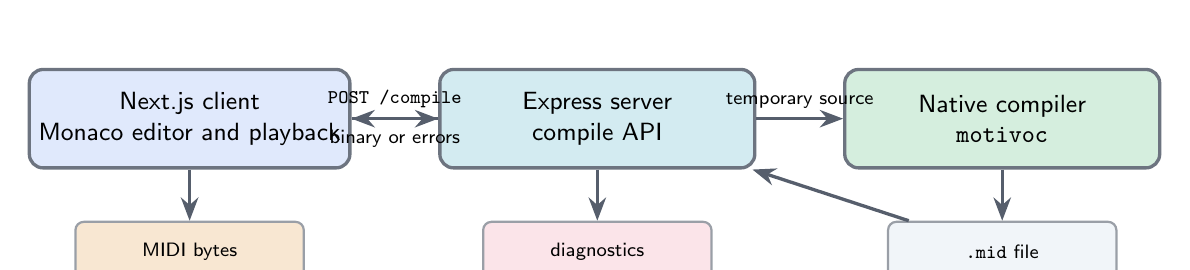
\begin{tikzpicture}[
      service/.style={rounded corners=5pt, draw=motivoInk!65, very thick, minimum width=4.0cm, minimum height=1.25cm,
      align=center, font=\small\sffamily},
      file/.style={rounded corners=3pt, draw=motivoInk!45, thick, minimum width=2.9cm, minimum height=0.75cm,
      align=center, font=\scriptsize\sffamily},
      arrow/.style={-Stealth, very thick, draw=motivoInk!75}
    ]
    \node[service, fill=motivoBlue!14] (client) {Next.js client\\Monaco editor and playback};
    \node[service, fill=motivoCyan!18, right=1.1cm of client] (server) {Express server\\compile API};
    \node[service, fill=motivoGreen!18, right=1.1cm of server] (compiler) {Native compiler\\\texttt{motivoc}};

    \node[file, fill=motivoAmber!18, below=0.65cm of client] (midi) {MIDI bytes};
    \node[file, fill=motivoRose!12, below=0.65cm of server] (diag) {diagnostics};
    \node[file, fill=motivoSoft, below=0.65cm of compiler] (midfile) {\texttt{.mid} file};

    \draw[arrow] (client) -- node[above, font=\scriptsize\sffamily] {\texttt{POST /compile}} (server);
    \draw[arrow] (server) -- node[above, font=\scriptsize\sffamily] {temporary source} (compiler);
    \draw[arrow] (compiler) -- (midfile);
    \draw[arrow] (midfile) -- (server);
    \draw[arrow] (server) -- node[below, font=\scriptsize\sffamily] {binary or errors} (client);
    \draw[arrow] (server) -- (diag);
    \draw[arrow] (client) -- (midi);
  \end{tikzpicture}
  \caption{Motivo Studio runtime architecture.
    The browser does not compile C++ code directly; it delegates compilation to the
  server.}\label{fig:studio-architecture}
\end{figure}

The frontend is organized by feature directories.
The editor feature wraps Monaco, registers Motivo language tokens, defines light and dark themes, and maps compiler
diagnostics into Monaco markers.
The compile feature owns the HTTP client and the response types.
The MIDI feature parses generated binary data into browser-side structures.
The piano-roll feature renders note rectangles on a canvas.
The playback feature schedules browser audio and exposes controls for play, stop, progress, and MIDI download.
This feature-oriented layout keeps UI responsibilities closer to their domain than a flat component directory would.

While the core contribution of this thesis is the compiler, a web-based \textit{Playground} was developed to demonstrate
the language's capabilities and provide an intuitive environment for composition.
The playground integrates the C++ compiler into a modern full-stack web application.

\subsection{System Architecture}\label{detail-subsec:system-architecture}

The playground follows a distributed architecture:

\noindent \textbf{Frontend (Next.js).} A React-based interface that provides the editor and visualization tools.

\noindent \textbf{Backend (Express).} A Node.js API that acts as a bridge.
It receives Motivo source code from the client, invokes the C++ \texttt{motivoc} binary via a sub-process, and streams
the resulting MIDI file back to the browser.

\noindent \textbf{Integration.} The system is containerized using Docker, ensuring that the C++ environment (including
Bison/Flex runtimes) is identical across development and production.

The backend is smaller but equally important.
The Express app exposes \texttt{GET /health} and \texttt{POST /compile}.
The compile route validates the request body with Zod, writes the source code to a temporary \texttt{.motivo} file,
spawns \texttt{motivoc}, and returns either \texttt{audio/midi} bytes or structured diagnostics.
The diagnostics parser normalizes compiler output into severity, stage, message, and optional source location fields so
the browser can highlight the relevant source range.

\section{Compilation Request Flow}\label{sec:request-flow}

The request flow matters because it connects three different implementation languages: TypeScript in the client,
TypeScript in the server, and C++ in the compiler.
The boundary between them is intentionally narrow.
The client sends source text.
The server returns MIDI bytes or diagnostic data.
The compiler remains an executable process with a stable command-line interface.

\begin{figure}[htbp]
  \centering
  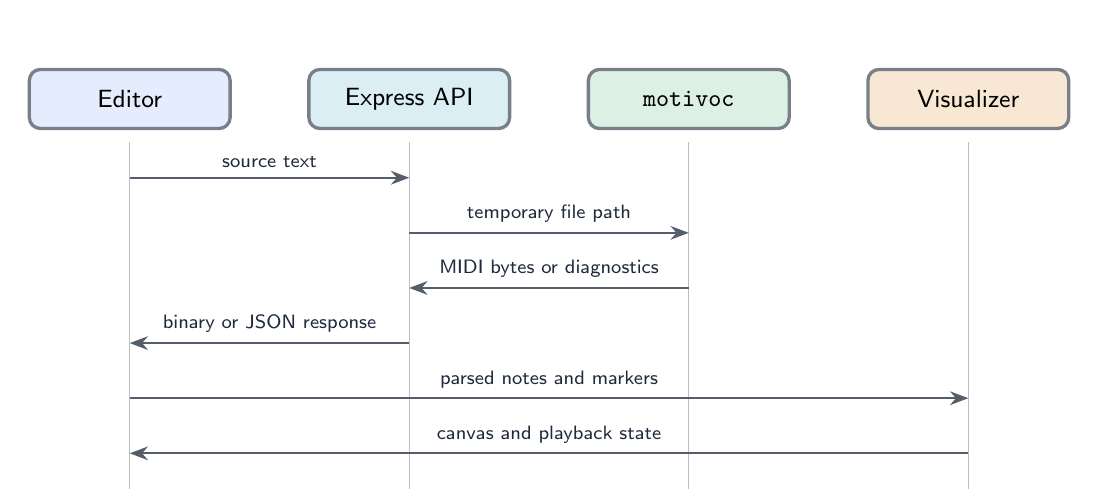
\begin{tikzpicture}[
      actor/.style={rounded corners=4pt, draw=motivoInk!60, very thick, minimum width=2.55cm, minimum height=0.75cm,
      align=center, font=\small\sffamily},
      msg/.style={font=\scriptsize\sffamily, text=motivoInk, align=center},
      arrow/.style={-Stealth, thick, draw=motivoInk!75}
    ]
    \node[actor, fill=motivoBlue!12] (editor) at (0,0) {Editor};
    \node[actor, fill=motivoCyan!15] (api) at (3.55,0) {Express API};
    \node[actor, fill=motivoGreen!15] (bin) at (7.1,0) {\texttt{motivoc}};
    \node[actor, fill=motivoAmber!18] (ui) at (10.65,0) {Visualizer};

    \foreach \x in {0,3.55,7.1,10.65} {
      \draw[draw=motivoInk!30] (\x,-0.55) -- (\x,-5.1);
    }

    \draw[arrow] (0,-1.0) -- node[msg, above] {source text} (3.55,-1.0);
    \draw[arrow] (3.55,-1.7) -- node[msg, above] {temporary file path} (7.1,-1.7);
    \draw[arrow] (7.1,-2.4) -- node[msg, above] {MIDI bytes or diagnostics} (3.55,-2.4);
    \draw[arrow] (3.55,-3.1) -- node[msg, above] {binary or JSON response} (0,-3.1);
    \draw[arrow] (0,-3.8) -- node[msg, above] {parsed notes and markers} (10.65,-3.8);
    \draw[arrow] (10.65,-4.5) -- node[msg, above] {canvas and playback state} (0,-4.5);
  \end{tikzpicture}
  \caption{Compile request sequence from editor action to browser visualization.}\label{fig:compile-sequence}
\end{figure}

This flow is not only a user-interface feature.
It is also a testable contract.
Server tests can replace the compiler binary with fake executables and verify success and failure handling without
requiring a native build.
Client tests can check diagnostic mapping, compile hooks, and visual components without invoking the C++ compiler.
Compiler tests remain native C++ tests focused on parsing, semantic analysis, lowering, MIDI writing, and golden
diagnostic behavior.

\section{Editor, Visualization, and Playback}\label{sec:editor-visualization}

The editor uses Monaco because it provides language registration, tokenization, themes, keyboard actions, and marker
support in a browser editor widget~\cite{Microsoft_Monaco_2026}.
Motivo Studio registers a Motivo language identifier and a Monarch tokenizer for language keywords, instruments, drum
notes, note literals, comments, and operators.
When compilation fails, diagnostics are converted into markers so the source location is visible inside the editor
rather than only in a log panel.

\subsection{IDE Integration and Diagnostics}\label{detail-subsec:ide-integration-and-diagnostics}

The playground features an IDE-like experience powered by the Monaco Editor.
A custom ``Monarch'' tokenizer was implemented for Motivo to provide syntax highlighting for musical keywords, pitch
literals, and control flow.

The most significant integration is the \textit{Diagnostics Feedback Loop}.
When a compilation fails, the Express server parses the structured error output from the compiler and returns it to the
client.
The React application then converts these diagnostics into Monaco ``Markers'', which underline the erroneous code and
display the compiler's semantic or syntax error messages in a tooltip.
This real-time feedback is enabled by the fast local compilation times discussed in the evaluation chapter.

The piano roll exists because MIDI is symbolic.
A successful compile response is not audio; it is a binary event file.
The browser parses that MIDI data and renders note events as colored rectangles against a piano-style vertical scale and
a horizontal time axis.
This view gives the user a visual check on timing, density, and pitch range before listening.
The playback layer uses browser audio libraries and SoundFont-based instruments to audition the
result~\cite{ToneJS_2026,SoundFontPlayer_2026}.
The rendered view and playback controls make Motivo Studio a practical development surface for the compiler.

\subsection{The Piano Roll and Synthesis}\label{detail-subsec:the-piano-roll-and-synthesis}

To visualize the composition, a custom \textit{Piano Roll} component was built using the HTML5 Canvas API\@.
Upon a successful compilation, the browser parses the returned MIDI bytes and renders them as colored rectangles on a
scrolling timeline.

The synthesis engine utilizes the \textit{Tone.js} library.
Because MIDI files contain only instructions and no sound, the playground loads a set of high-quality
\textit{Soundfonts} representing General MIDI instruments.
The playback logic schedules notes in the browser's audio context, allowing the user to hear their ``coded'' composition
instantly.
The synchronization between the scrolling piano roll and the audio playback is maintained through a high-precision
request-animation-frame loop, ensuring a professional and ``alive'' feel to the prototype.

\begin{figure}[p]
  \centering
  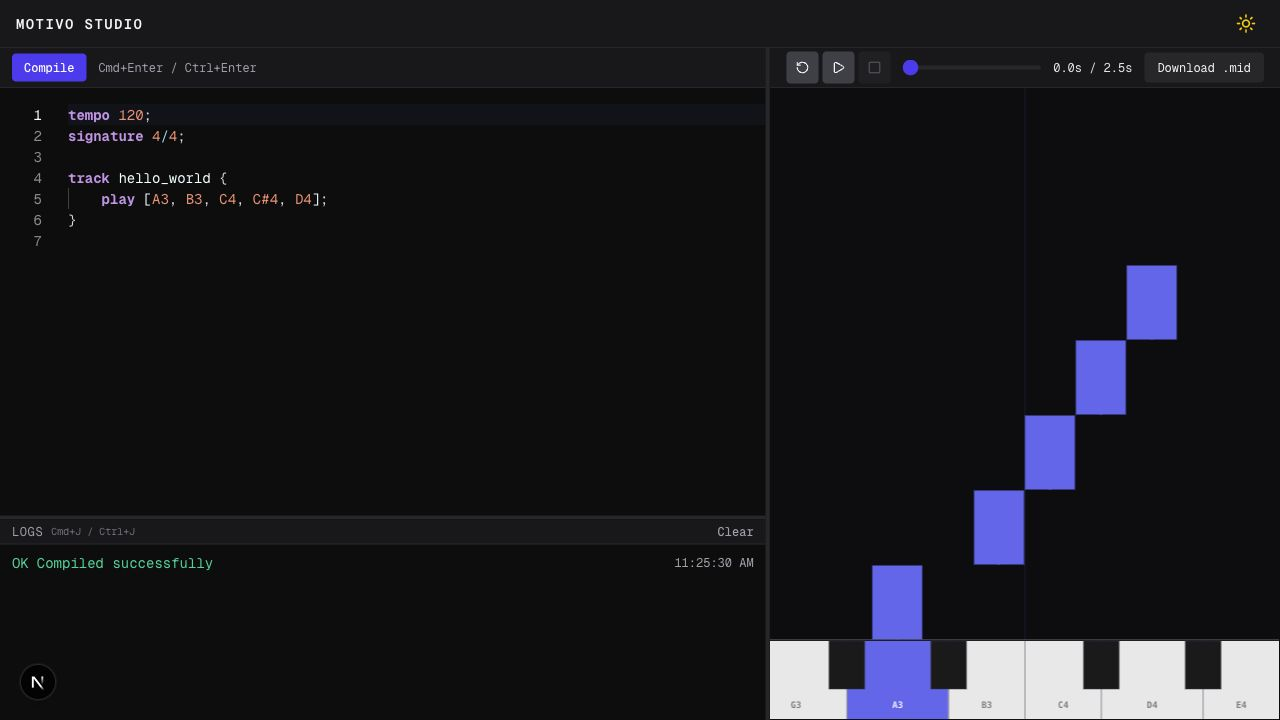
\includegraphics[width=\textwidth]{assets/screenshots/motivo-studio-success.png}
  \caption{Motivo Studio after a successful local compile.
    The screenshot shows the Monaco editor, success log, playback controls, and generated piano-roll
    visualization for the
  default Motivo snippet.}\label{fig:studio-success-screenshot}
\end{figure}

\begin{figure}[htbp]
  \centering
  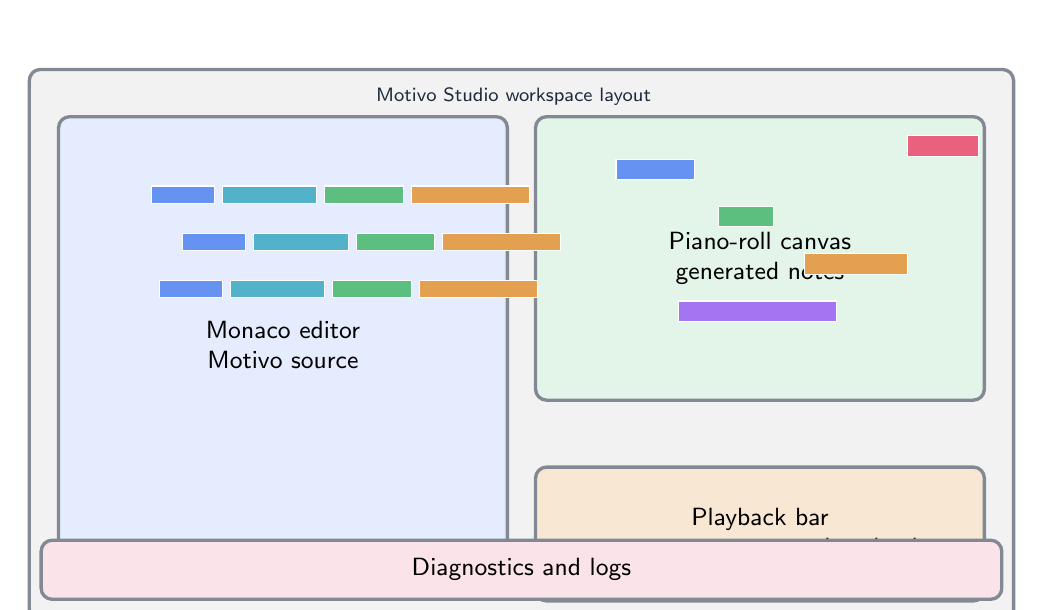
\begin{tikzpicture}[
      panel/.style={rounded corners=4pt, draw=motivoInk!55, very thick, align=center, font=\small\sffamily},
      small/.style={font=\scriptsize\sffamily, text=motivoInk}
    ]
    \node[panel, fill=motivoInk!6, minimum width=12.5cm, minimum height=7.0cm] (shell) {};
    \node[panel, fill=motivoBlue!12, minimum width=5.7cm, minimum height=5.8cm, anchor=west] at (-5.9,0)
    {Monaco editor\\Motivo source};
    \node[panel, fill=motivoGreen!12, minimum width=5.7cm, minimum height=3.6cm, anchor=east] at (5.9,1.1)
    {Piano-roll canvas\\generated notes};
    \node[panel, fill=motivoAmber!18, minimum width=5.7cm, minimum height=1.7cm, anchor=east] at (5.9,-2.4)
    {Playback bar\\transport, progress, download};
    \node[panel, fill=motivoRose!12, minimum width=12.2cm, minimum height=0.75cm, anchor=south] at (0,-3.25)
    {Diagnostics and logs};

    \foreach \x/\w/\c in {-4.7/0.8/motivoBlue,-3.8/1.2/motivoCyan,-2.5/1.0/motivoGreen,-1.4/1.5/motivoAmber} {
      \draw[fill=\c!70, draw=white] (\x,1.8) rectangle ++(\w,0.22);
      \draw[fill=\c!70, draw=white] (\x+0.4,1.2) rectangle ++(\w,0.22);
      \draw[fill=\c!70, draw=white] (\x+0.1,0.6) rectangle ++(\w,0.22);
    }
    \draw[fill=motivoBlue!70, draw=white] (1.2,2.1) rectangle ++(1.0,0.26);
    \draw[fill=motivoGreen!70, draw=white] (2.5,1.5) rectangle ++(0.7,0.26);
    \draw[fill=motivoAmber!70, draw=white] (3.6,0.9) rectangle ++(1.3,0.26);
    \draw[fill=motivoRose!70, draw=white] (4.9,2.4) rectangle ++(0.9,0.26);
    \draw[fill=motivoViolet!70, draw=white] (2.0,0.3) rectangle ++(2.0,0.26);
    \node[small] at (-0.1,3.15) {Motivo Studio workspace layout};
  \end{tikzpicture}
  \caption{Motivo Studio workspace organization.
    The figure summarizes the editor, visualization, playback, and diagnostics surfaces implemented in the
  client.}\label{fig:studio-workspace}
\end{figure}

\section{Deployment and Runtime Configuration}\label{sec:deployment}

The local production-like stack is defined by Docker Compose.
The server image builds the C++ compiler and installs \texttt{motivoc} at \texttt{/usr/local/bin/motivoc}.
The client image builds the Next.js application and proxies API requests to the server inside the Compose network.
The nginx gateway terminates HTTPS with a local self-signed certificate and routes browser traffic to the client and
API routes to the server.
Docker is used here as a reproducibility tool: it keeps the compiler, server, and client runtime assumptions explicit
instead of relying on an ad hoc local machine setup~\cite{Docker_2026}.

\begin{figure}[htbp]
  \centering
  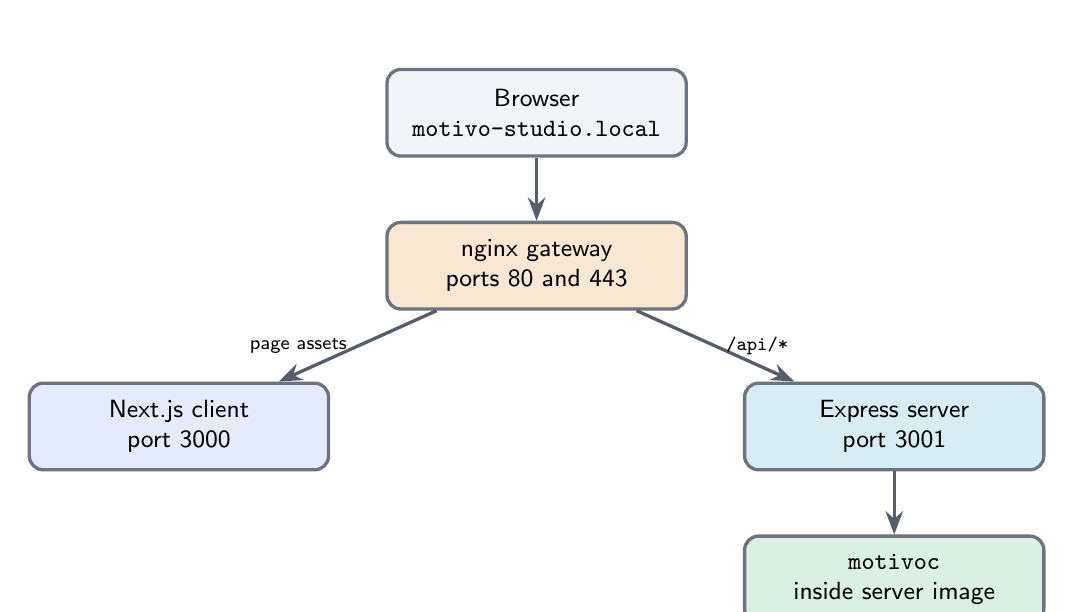
\begin{tikzpicture}[
      svc/.style={rounded corners=5pt, draw=motivoInk!65, very thick, minimum width=3.8cm, minimum height=1.1cm,
      align=center, font=\small\sffamily},
      arrow/.style={-Stealth, very thick, draw=motivoInk!75}
    ]
    \node[svc, fill=motivoSoft] (browser) {Browser\\\texttt{motivo-studio.local}};
    \node[svc, fill=motivoAmber!18, below=0.8cm of browser] (nginx) {nginx gateway\\ports 80 and 443};
    \node[svc, fill=motivoBlue!13, below left=0.9cm and 0.7cm of nginx] (client) {Next.js client\\port 3000};
    \node[svc, fill=motivoCyan!16, below right=0.9cm and 0.7cm of nginx] (server) {Express server\\port 3001};
    \node[svc, fill=motivoGreen!16, below=0.8cm of server] (compiler) {\texttt{motivoc}\\inside server image};

    \draw[arrow] (browser) -- (nginx);
    \draw[arrow] (nginx) -- node[left, font=\scriptsize\sffamily] {page assets} (client);
    \draw[arrow] (nginx) -- node[right, font=\scriptsize\sffamily] {\texttt{/api/*}} (server);
    \draw[arrow] (server) -- (compiler);
  \end{tikzpicture}
  \caption{Docker Compose deployment topology for Motivo Studio.}\label{fig:deployment}
\end{figure}

Configuration is intentionally small.
The server reads \texttt{PORT}, \texttt{HOSTNAME}, and \texttt{COMPILER\_BIN}.
The client uses \texttt{API\_PROXY\_URL} for API rewrites.
This is sufficient for the current deployment model, where the compiler is a local executable reachable by the API
container.
Future remote compilation would require a different trust and resource model, but that is outside the present thesis.

\section{Testing and Continuous Integration}\label{sec:testing-ci}

The project uses separate CI workflows for the paper, compiler, server, and client through GitHub Actions
workflows~\cite{GitHub_Actions_2026}.
The paper workflow checks LaTeX formatting, spelling, linting, and PDF build.
The compiler workflow checks formatting, builds the native compiler, runs CTest with GoogleTest, publishes test reports,
and summarizes coverage through gcovr.
The server and client workflows run ESLint, TypeScript type checks, Prettier checks, Vitest tests with coverage, builds,
and Docker image packaging.

\begin{figure}[htbp]
  \centering
  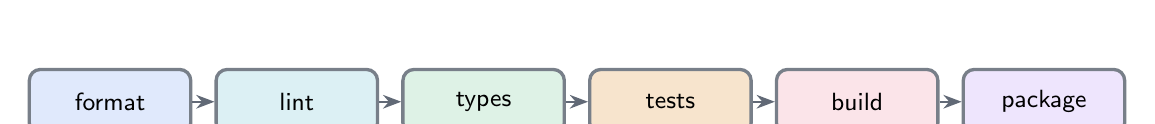
\begin{tikzpicture}[
      job/.style={rounded corners=4pt, draw=motivoInk!60, very thick, minimum width=2.05cm, minimum height=0.82cm,
      align=center, font=\small\sffamily},
      arrow/.style={-Stealth, thick, draw=motivoInk!70}
    ]
    \node[job, fill=motivoBlue!14] (format) {format};
    \node[job, fill=motivoCyan!14, right=0.28cm of format] (lint) {lint};
    \node[job, fill=motivoGreen!14, right=0.28cm of lint] (types) {types};
    \node[job, fill=motivoAmber!20, right=0.28cm of types] (test) {tests};
    \node[job, fill=motivoRose!12, right=0.28cm of test] (build) {build};
    \node[job, fill=motivoViolet!13, right=0.28cm of build] (package) {package};

    \draw[arrow] (format) -- (lint);
    \draw[arrow] (lint) -- (types);
    \draw[arrow] (types) -- (test);
    \draw[arrow] (test) -- (build);
    \draw[arrow] (build) -- (package);
  \end{tikzpicture}
  \caption{Common CI progression used across the project, adapted per component.}\label{fig:ci-flow}
\end{figure}

The test suites cover different failure modes.
Compiler unit tests use GoogleTest and exercise note mapping, parsing, semantic rules, lowering expressions, cursor
behavior, pattern calls, voice parallelism, and MIDI writing~\cite{GoogleTest_2026}.
Golden tests check representative success and error fixtures.
Server and client tests use Vitest to cover request validation, controller behavior, compiler process integration,
diagnostics parsing, editor setup, MIDI parsing, playback utilities, piano-roll rendering, shared UI components, and IDE
workflow hooks~\cite{Vitest_2026}.
This distribution is appropriate for a full-stack compiler tool because failures can happen at several
boundaries: language semantics, binary serialization, process execution, HTTP transport, browser parsing, and
UI rendering.

To ensure the correctness of the compilation pipeline and the validity of the generated MIDI artifacts, a comprehensive
testing suite was implemented using the \textit{Google Test} framework.
The testing strategy follows a tiered approach, covering individual units, module boundaries, and end-to-end
integration.

\subsection{Unit Testing}\label{detail-subsec:unit-testing}

Unit tests focus on the smallest verifiable components of the compiler.
This is particularly important for the musical domain logic, where small errors in calculation can lead to significant
musical dissonance.
The test cases cover several error-prone responsibilities.

\noindent \textbf{Pitch Math.} Verifying that pitch literals (e.g., \texttt{A4}) map correctly to MIDI note
numbers (e.g.,
69) and that octave offsets are handled according to the standard.

\noindent \textbf{Diagnostic Reporting.} Ensuring that the \texttt{DiagnosticsEngine} correctly captures and formats
errors across different stages of the pipeline.

\noindent \textbf{Lexer Accuracy.} Stress-testing the Flex regex patterns with edge cases, such as multiple consecutive
accidentals or varying whitespace.

\subsection{Integration and Regression Testing}\label{detail-subsec:integration-and-regression-testing}

Integration tests verify that the different stages of the compiler work together seamlessly.
These tests utilize a ``Golden File'' methodology:

\noindent A set of representative Motivo source files (located in \texttt{tests/data/}) is compiled.

\noindent The resulting IR is checked for temporal consistency (e.g., ensuring no notes overlap unless explicitly
requested).

\noindent The final MIDI binary is compared against a previously validated ``golden'' version to detect
unexpected changes
in behavior.

Regression tests were instrumental during the refactoring process (e.g., when decomposing the monolithic lowerer).
By maintaining a suite of complex compositions---such as the \texttt{fur\_elise.motivo} example---the compiler's
output could be
verified for byte-level consistency after every architectural change.

\subsection{Integration in the Development Lifecycle}\label{detail-subsec:integration-in-the-development-lifecycle}

The testing suite is integrated into the build system via CMake's \texttt{CTest} module.
This allows for one-command verification of the entire system (\texttt{make test}).
By enforcing a high level of test coverage, particularly in the lowering and backend stages, the implementation provides
repeatable evidence that the generated compositions are mathematically and musically accurate.
This verification process supports the thesis by treating the creative tool as a repeatable software system.

\begin{table}[htbp]
  \centering
  \renewcommand{\arraystretch}{1.3}
  \begin{tabularx}{\textwidth}{>{\raggedright\arraybackslash}p{2.8cm}>{\raggedright\arraybackslash}p{3.2cm}X}
    \toprule
    \textbf{Subsystem} & \textbf{Primary tools} & \textbf{What the tests protect} \\
    \midrule
    Compiler & CTest and GoogleTest & Grammar behavior, semantic diagnostics, lowering, MIDI writer, golden fixtures. \\
    Server & Vitest and Supertest & Request validation, compile route behavior, fake compiler integration,
    diagnostics parsing. \\
    Client & Vitest and Testing Library & Editor wiring, MIDI parsing, piano-roll rendering, playback hooks,
    IDE components. \\
    Paper & latexmk, tex-fmt, lint, codespell & Formatting, spelling, LaTeX warnings, and reproducible PDF
    generation. \\
    \bottomrule
  \end{tabularx}
  \caption{Testing responsibilities by subsystem.}\label{tab:testing-matrix}
\end{table}

This engineering chapter completes the description of the implemented system.
The next chapter evaluates Motivo through local measurements and source-to-output comparisons.

\chapter{Empirical Evaluation}\label{ch:evaluation}

The evaluation is designed around claims that can be supported by the implementation.
Motivo is not evaluated as a general measure of musical creativity, and the thesis does not include a user study.
Instead, this chapter evaluates engineering properties: whether the compiler can expand compact source programs into
larger MIDI event streams, how quickly it compiles a small benchmark corpus on one local machine, what safety limits the
current implementation imposes, and how the software project is tested.

\section{Methodology}\label{sec:evaluation-methodology}

The benchmark was run locally with a Release build of \texttt{motivoc}.
The binary was built outside the repository at \texttt{/tmp/motivo-thesis-bench-build} using CMake 4.3.2 and Apple
clang 21.0.0.
Measurements were taken on an Apple M3 Pro machine with 18 GB of RAM\@.
The timing tool was \texttt{hyperfine} 1.20.0 with shell execution disabled, 5 warmup runs, and 50 measured
runs~\cite{Hyperfine_2026}.
Each measured command compiled one \texttt{.motivo} source file and wrote the resulting MIDI file, so the
results include
process startup, parsing, semantic analysis, lowering, MIDI serialization, and file output.

The benchmark corpus was synthetic.
It was built to exercise source-to-event expansion rather than to produce musically refined pieces.
This distinction matters.
A loop that generates 20,000 notes is useful for measuring expansion and compilation cost, but it does not prove that
the generated score is artistically interesting.
The benchmark therefore supports the engineering claim that Motivo can generate many symbolic events from
compact source rules within the tested limit.

A defining characteristic of the Motivo compiler is its ``zero-runtime'' architecture, which shifts the
computational burden entirely to the compilation phase.
To evaluate the viability of this approach, it is essential to analyze the compiler's execution speed, particularly as
the complexity of the musical composition scales.

\subsection{Theoretical Complexity}\label{detail-subsec:theoretical-complexity}

The compilation pipeline is composed of several sequential passes, each with a distinct computational complexity:

\noindent \textbf{Frontend and Semantic Analysis.} The complexity of parsing and type-checking is proportional to the
number of lines of source code, $O(S)$, where $S$ is the size of the abstract syntax tree.
Because these passes do not unroll loops or instantiate patterns multiple times, they remain extremely fast
regardless of the composition's length.

\noindent \textbf{Lowering Engine.} The unrolling process has a time complexity of $O(E)$, where $E$ is the total number
of generated \texttt{NoteEvent}s. A simple \texttt{loop (1000)} statement will execute its body 1,000 times during
this phase, meaning the lowering time is proportional to the density of the final timeline, not the brevity of the
source code.

\noindent \textbf{MIDI Backend.} The backend must sort the absolute events by their tick values before computing
delta-times.
This stable sort introduces a time complexity of $O(E \log E)$.
Serializing the events into the binary file requires a final linear pass, $O(E)$.

Therefore, the overall time complexity of the compilation process is bounded by the sorting phase in the backend:
$O(E \log E)$.

\section{Compilation Time}\label{sec:compile-time}

Table~\ref{tab:benchmark-results} shows the measured results.
The fastest case and the realistic example are close to 2 ms.
The largest synthetic cases are around 6 ms.
Because these times are small, they should be interpreted as local measurements on the stated machine rather than as a
portable performance result.
They are still useful for the thesis because they show that the current native compiler is fast enough to support an
interactive compile loop in this local setup.

\begin{table}[htbp]
  \centering
  \footnotesize
  \renewcommand{\arraystretch}{1.25}
  \begin{tabular}{lrrrrr}
    \toprule
    \textbf{Program} & \textbf{LOC} & \textbf{Note events} & \textbf{MIDI size} & \textbf{Mean ms} & \textbf{SD ms} \\
    \midrule
    \texttt{single\_loop\_100} & 7 & 100 & 856 B & 2.02 & 0.31 \\
    \texttt{single\_loop\_1000} & 7 & 1,000 & 8,056 B & 2.14 & 0.31 \\
    \texttt{single\_loop\_10000} & 7 & 10,000 & 80,056 B & 3.96 & 0.24 \\
    \texttt{single\_loop\_20000} & 7 & 20,000 & 160,056 B & 6.03 & 0.15 \\
    \texttt{chord\_loop\_5000} & 7 & 20,000 & 160,056 B & 5.90 & 0.17 \\
    \texttt{drum\_groove\_500} & 18 & 10,000 & 88,053 B & 6.39 & 0.19 \\
    \texttt{example\_copy} & 77 & 188 & 1,751 B & 2.04 & 0.18 \\
    \bottomrule
  \end{tabular}
  \caption{Local Release-build compilation benchmark.
  Times include MIDI file writing and are based on 50 measured runs after 5 warmups.}\label{tab:benchmark-results}
\end{table}

\begin{figure}[htbp]
  \centering
  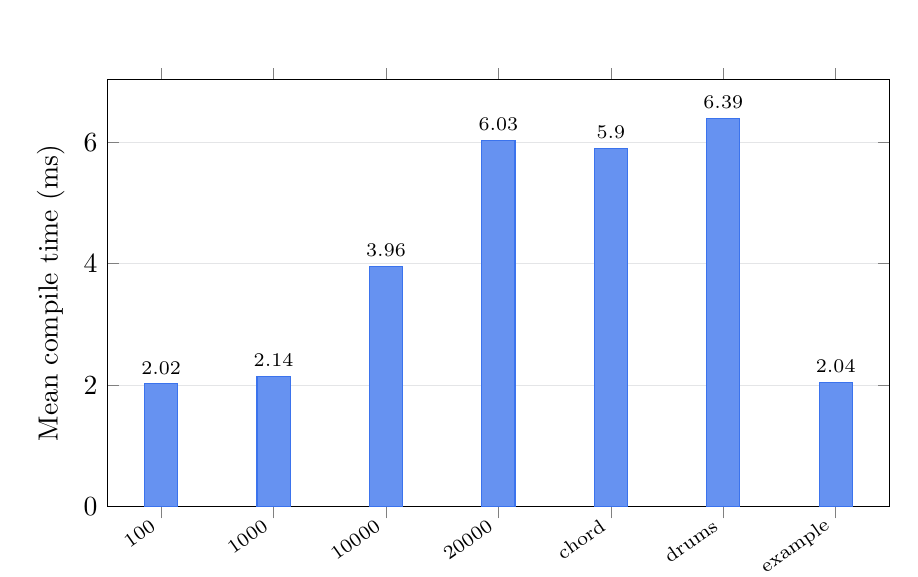
\begin{tikzpicture}
    \begin{axis}[
        ybar,
        width=0.95\textwidth,
        height=7cm,
        ymin=0,
        ylabel={Mean compile time (ms)},
        symbolic x coords={100,1000,10000,20000,chord,drums,example},
        xtick=data,
        x tick label style={rotate=35, anchor=east, font=\scriptsize},
        nodes near coords,
        nodes near coords style={font=\scriptsize},
        bar width=12pt,
        enlarge x limits=0.08,
        ymajorgrids=true,
        grid style={draw=motivoInk!12}
      ]
      \addplot[fill=motivoBlue!70, draw=motivoBlue!90] coordinates {
        (100,2.02)
        (1000,2.14)
        (10000,3.96)
        (20000,6.03)
        (chord,5.90)
        (drums,6.39)
        (example,2.04)
      };
    \end{axis}
  \end{tikzpicture}
  \caption{Mean compile times for the local benchmark corpus.}\label{fig:benchmark-time}
\end{figure}

The near-linear growth in the single-loop cases is consistent with the implementation.
Parsing and semantic analysis see a small source program, while lowering and MIDI writing scale with the number of
generated events.
The backend also sorts events by tick before computing delta-times.
The result is still small at the current safety limit, but the implementation should not be described as unbounded.

\subsection{Execution Speed and Real-Time Viability}\label{detail-subsec:execution-speed-and-real-time-viability}

Because the compiler is implemented as a native C++23 program without reliance on garbage collection or dynamic dispatch
for AST traversal, the constant factors in the time complexity are small in the current measurements.
In practice, the compiler generates compositions containing event streams up to the current implementation
limit in a fraction of a second.

These local measurements are relevant to Motivo Studio because the editor workflow depends on compilation
remaining quick enough for interactive use.
The interactive playground environment (discussed in previous chapters) relies on the compiler's ability to re-compile
the entire source file during interactive compile actions.
Because the execution time for typical musical pieces (ranging from hundreds to thousands of events) sits
well below the latency usually noticed during ordinary editor interaction, the composer experiences
interactive auditory and visual feedback without using an interpreted runtime during playback.

\section{Source-to-Event Expansion}\label{sec:compression}

A major objective of Motivo is to provide a highly expressive interface for music composition,
reducing the manual effort required to construct complex arrangements.
We evaluate this expressiveness by analyzing the ``compression ratio''---the difference between the amount of
code written
by the composer and the number of low-level MIDI events generated by the compiler.

\subsection{Algorithmic Conciseness}\label{detail-subsec:algorithmic-conciseness}

Traditional MIDI sequencers and digital audio workstations require the composer to manually place every note on a grid.
In contrast, Motivo allows composers to define structural rules and relationships.

Consider the following drum pattern from the \texttt{example.motivo} file:
\begin{lstlisting}[language=Motivo, caption={A generative drum pattern using control flow.},label={lst:evaluation-drum-pattern}]
track percussion using drums {
    pattern groove() {
        for (let i = 0; i < 16; i = i + 1) {
            play hihat from i;
            if (i % 8 == 0) { play kick from i; }
            if (i % 8 == 4) { play snare from i; }
        }
    }
    loop (3) { play groove(); }
}
\end{lstlisting}

This 10-line block of code encapsulates a complex rhythm.
The \texttt{for} loop defines the underlying hi-hat grid, while the modulo-based \texttt{if} conditions procedurally
generate the kick and snare syncopation.
The \texttt{loop (3)} statement then instantiates this 16-beat pattern three times across the timeline.

\subsection{The Compression Ratio}\label{detail-subsec:the-compression-ratio}

To achieve the same result in a traditional MIDI editor, the composer would have to manually draw 48 hi-hat notes, 6
kick drum notes, and 6 snare drum notes---a total of 60 individual note events, which translates to 120 low-level MIDI
messages (\texttt{Note-On} and \texttt{Note-Off}).

Motivo abstracts these 120 MIDI messages into just a handful of declarative rules.
The resulting ``compression ratio'' is exceedingly high.
As the composition grows---for example, looping the groove 32 times instead of 3---the size of Motivo source
code remains
completely unchanged, while the output scales to hundreds or thousands of events.

This expressiveness validates the core thesis: by shifting from a linear, event-based representation to a structural,
programming-based representation, the manual overhead of repetitive event placement can be reduced.
The composer can focus on higher-level musical structure while the lowering engine handles repetitive
temporal event placement.

The main measured expressiveness result is source-to-event expansion.
The 20,000-event single-loop program uses 7 lines of source.
The chord-loop program also uses 7 lines and generates 20,000 note events because each loop iteration emits a
four-note chord.
The 18-line drum groove generates 10,000 note events by combining a 16-step bar pattern with a 500-iteration loop.
These examples demonstrate the intended effect of the language: repeated symbolic structure remains compact in source
form while the compiler expands it into explicit event data.

\begin{figure}[htbp]
  \centering
  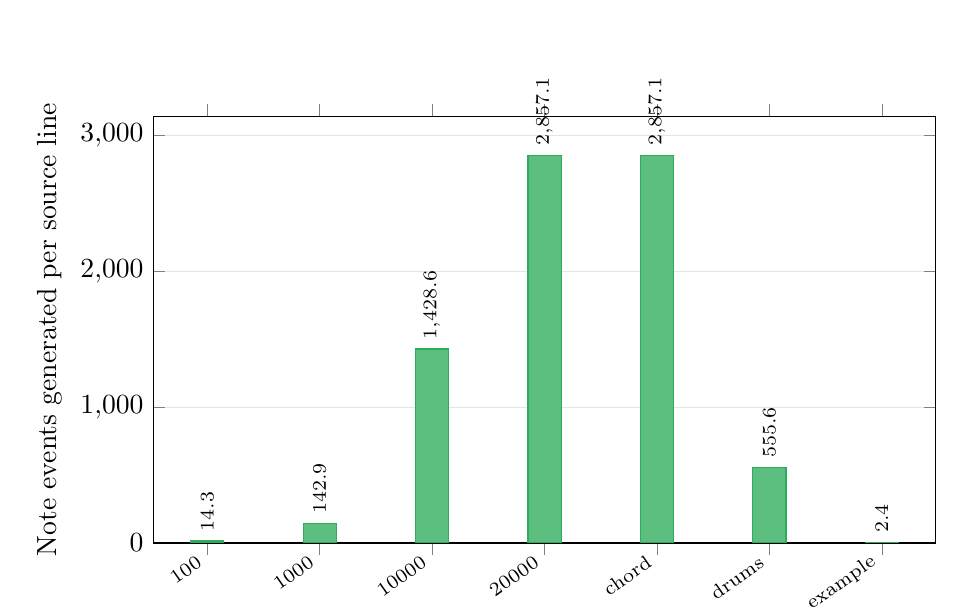
\begin{tikzpicture}
    \begin{axis}[
        ybar,
        width=0.95\textwidth,
        height=7cm,
        ymin=0,
        ylabel={Note events generated per source line},
        symbolic x coords={100,1000,10000,20000,chord,drums,example},
        xtick=data,
        x tick label style={rotate=35, anchor=east, font=\scriptsize},
        nodes near coords,
        nodes near coords style={font=\scriptsize, rotate=90, anchor=west},
        bar width=12pt,
        enlarge x limits=0.08,
        ymajorgrids=true,
        grid style={draw=motivoInk!12}
      ]
      \addplot[fill=motivoGreen!70, draw=motivoGreen!90] coordinates {
        (100,14.3)
        (1000,142.9)
        (10000,1428.6)
        (20000,2857.1)
        (chord,2857.1)
        (drums,555.6)
        (example,2.4)
      };
    \end{axis}
  \end{tikzpicture}
  \caption{Source-to-event expansion in the benchmark corpus.}\label{fig:compression-chart}
\end{figure}

This metric should not be overinterpreted.
More generated events per source line is useful when the source expresses meaningful repetition, but it can also produce
uninteresting repetition.
For a bachelor thesis, the metric is still valuable because it connects the language design to a measurable output.
The compiler removes repetitive manual event placement from the source program and makes the expansion explicit in the
MIDI artifact.

\section{Current Limits and Failure Behavior}\label{sec:limits}

The most important current limit is the event cap in the lowerer.
\texttt{MAX\_EVENTS} is 20,000.
A program that generates 20,001 note events fails during lowering with the diagnostic
\texttt{program exceeds 20000 event limit (has 20001)}.
This is a deliberate safety boundary in the implementation.
It prevents runaway programs from producing very large event streams, but it also means the thesis should not claim that
Motivo currently supports arbitrarily large scores.

The benchmark also revealed a language consistency issue in an old example file.
The current parser does not accept a key-signature header, and key signatures are not part of the current language.
The temporary benchmark copy of the example removed that unsupported line.
The thesis therefore treats key-signature and harmonic-context support as future work, not as implemented behavior.

Single-run memory checks with macOS \texttt{/usr/bin/time -l} reported maximum resident set sizes in the range of
approximately 5.2 MB to 7.8 MB for the largest synthetic cases.
This is useful as an informal local observation, but the time benchmark is the stronger measurement because it was run
with repeated trials.
The memory result should be described cautiously if used outside this chapter.

\subsection{Memory Footprint}\label{detail-subsec:memory-footprint}

The value-oriented design of the AST and IR ensures that the compiler's memory footprint remains minimal.
The use of \texttt{std::variant} supports spatial locality in the CPU cache during AST traversal.
The intermediate representation holds only the necessary atomic data (pitch, start beat, duration, velocity) packed
tightly into \texttt{struct}s. Consequently, even a composition unrolled into large event streams within the
configured implementation limits will consume only a few
megabytes of RAM, allowing the compiler to run seamlessly on low-end hardware or within memory-constrained Docker
containers.

\section{Testing Evidence}\label{sec:test-evidence}

The repository contains a broad test suite across compiler, server, and client components.
The native compiler build used during earlier local inspection exposed 582 CTest-discovered tests.
The server Vitest report in the workspace recorded 20 passing tests across 10 suites, and the client Vitest report
recorded 54 passing tests across 38 suites.
The same reports showed server line coverage of 97.95\% and client line coverage of 89.46\%.
These values should be regenerated before final submission, but they provide a useful snapshot of the current testing
discipline.

Coverage is not a proof of correctness.
It does not show whether the language is pleasant to use or whether every musical edge case has been modeled.
It does show that the implementation is treated as a software system with repeatable checks.
For this thesis, that matters because Motivo is evaluated both as a language design and as a full-stack engineering
project.

\section{Comparative Interpretation}\label{sec:comparative-interpretation}

To fully evaluate the utility and positioning of Motivo, it must be contextualized within the existing
ecosystem of music programming tools.
This section provides a comparative analysis against two distinct paradigms: live-coding environments (exemplified by
Sonic Pi) and low-level scripting libraries (such as Python's \texttt{mido}).

\subsection{Comparison with Sonic Pi}\label{detail-subsec:comparison-with-sonic-pi}

Sonic Pi is a highly successful live-coding language embedded in Ruby, designed primarily for performance and education.
While both Sonic Pi and Motivo allow music to be expressed as text, their underlying design philosophies lead
to different compositional workflows.

\subsubsection{Execution Model}
Sonic Pi utilizes a real-time, interpreted execution model.
The musician writes scripts that trigger sounds ``on the fly'' through the SuperCollider synthesis engine.
Time is managed explicitly by the programmer using the \texttt{sleep} function, which halts the execution thread.

In contrast, Motivo is fully compiled and ``zero-runtime''.
There is no concept of a thread sleeping; instead, the \texttt{play} and \texttt{rest} commands define a mathematical
relationship on a static timeline.
While Sonic Pi excels in improvisational settings where the code is meant to be modified while it runs,
Motivo is oriented toward \textit{structural composition}, where the composer needs a complex arrangement to
resolve into a consistently quantized MIDI file every time it is compiled.

\subsubsection{Structural Abstraction in Practice}
In Sonic Pi, polyphony and parallel execution are achieved by spawning new threads (e.g., using \texttt{in\_thread}).
This can lead to synchronization issues if the composer does not meticulously manage the timing of each thread.
Motivo resolves parallelism through the \texttt{voice} construct.
Because voices are unrolled at compile-time by isolating the internal cursor, the compiler supports that parallel
musical lines are aligned according to the compiler cursor model at their inception without requiring manual
thread management or timing arithmetic from the composer.

\subsection{Comparison with Raw MIDI Scripting}\label{detail-subsec:comparison-with-raw-midi-scripting}

For offline composition, many developers use general-purpose programming languages combined with MIDI libraries, such as
Python's \texttt{mido} or C++'s \texttt{RtMidi}.
While these tools offer absolute control over the output, they operate at an exceptionally low level of abstraction.

\subsubsection{Event Placement and Musical Intent}
When using a library like \texttt{mido}, the composer must manually construct \texttt{Note-On} and \texttt{Note-Off}
messages.
Crucially, because the MIDI file format relies on delta-times, the composer is forced to manually calculate the tick
difference between every sequential event across all tracks.

Motivo abstracts this entirely.
A composer writing \texttt{play (C4, E4, G4):2;} in Motivo communicates their \textit{musical intent}---playing a
C-Major triad for two beats.
Motivo's lowering engine and backend automatically handle the translation into absolute beats, the flattening into
individual notes, the sorting by absolute tick, and the final variable-length delta-time encoding.

\subsubsection{Boilerplate and Expressiveness}
A simple four-beat loop of a hi-hat playing eighth notes requires a significant amount of boilerplate in Python:
creating a file, creating a track, appending tempo metadata, and writing a loop that interleaves \texttt{Note-On} and
\texttt{Note-Off} messages with explicit delta times.

Motivo achieves the same result with minimal syntax:
\begin{lstlisting}[language=Motivo,label={lst:midi-scripting-comparison}]
tempo 120;
track using drums {
    loop (8) { play hihat :0.5; }
}
\end{lstlisting}

This contrast in verbosity illustrates Motivo's intended role as a domain-specific tool.
By embedding musical semantics (like default durations, rest tracking, and automatic track/channel assignment) directly
into the language design, the compiler reduces cognitive friction and allows the user to operate strictly within the
musical domain.

\section{Evaluation Summary}\label{sec:evaluation-summary}

The evaluation supports three bounded conclusions.
First, Motivo's compiler can expand compact source rules into much larger MIDI event streams, as shown by the synthetic
source-to-event benchmarks.
Second, the current Release build compiles the tested programs quickly on the local machine, with the largest benchmark
cases finishing around 6 ms.
Third, the implemented system includes testing and CI coverage across compiler, API, client, and paper workflows.

The evaluation also establishes limits.
The benchmark corpus is synthetic, the hardware is a single Apple M3 Pro machine, the compiler has a 20,000-note-event
safety cap, and no user study was performed.
These limits do not weaken the thesis; they make the claims more precise.
The project demonstrates a working compiler-centered music tool and measures its current behavior without claiming more
than the implementation can support.

\chapter{Conclusions and Future Directions}\label{ch:conclusion}

This thesis presented Motivo, a domain-specific language, native compiler, and web-based studio for offline symbolic
music composition.
The project began with a practical observation: repeated musical structures are often easier to describe as rules than
as copied note events.
Motivo turns that observation into a compiler pipeline.
The source program names musical values and procedures, the semantic analyzer validates the structure, the lowerer
expands it into timestamped events, and the MIDI writer serializes the result into a Standard MIDI File.

The work also demonstrates that the compiler can be embedded into a larger software product.
Motivo Studio connects the C++ compiler to a browser editor through an Express API, renders generated MIDI in a piano
roll, supports browser playback, and is packaged through Docker and nginx.
The project is therefore not only a small programming language experiment.
It is also a full-stack engineering exercise with component boundaries, automated tests, CI workflows, deployment
configuration, and a user-facing interface.

\section{Contributions}\label{sec:contributions}

The first contribution is the Motivo language model.
It provides a compact set of abstractions for notes, rests, chords, sequences, patterns, tracks, voices, and control
flow.
These abstractions are deliberately close to symbolic musical structure and deliberately far from raw MIDI byte
construction.
The language is small, but it is sufficient to express repeated arrangements and parallel lines in the current
implementation.

The second contribution is the compiler architecture.
The implementation uses a conventional staged pipeline: scanner, parser, semantic analyzer, lowerer, and backend.
The most project-specific part is the cursor-based lowering model.
That model lets sequential statements advance musical time, explicit offsets place events without changing the main
cursor, voices run with isolated cursors, and pattern calls return reconstructed musical values.
This is the core mechanism that connects source-level structure to MIDI note events.

The third contribution is Motivo Studio.
The application shows how the compiler can be made accessible through a web interface.
The editor, diagnostics loop, MIDI parsing, piano-roll visualization, playback controls, server wrapper, Docker stack,
and CI workflows demonstrate the software engineering side of the project.
For a bachelor's thesis, this part is important because it shows that the work is not only theoretical.
It is an implemented system with several interacting modules.

The same contribution can also be viewed through the structural abstractions implemented by the compiler. The
language provides constructs such as \texttt{pattern}, \texttt{track}, and \texttt{voice}, which allow
polyphonic arrangements to be described without manually calculating absolute timestamps or delta-times. The
deterministic lowering algorithm connects those abstractions to a static intermediate representation, while
the semantic analyzer checks type and structural constraints before MIDI generation.

The fourth contribution is the empirical evaluation.
The local benchmark results show that Motivo can generate large symbolic event streams from compact source programs and
compile them quickly in the tested Release configuration.
The results are intentionally bounded by the current implementation and hardware.
They support the practical claim that Motivo is suitable for interactive local experimentation at the current scale.

\section{Limitations}\label{sec:limitations}

Motivo is not a complete composition environment.
It does not provide audio synthesis inside the compiler.
It does not model performer expression beyond the simple event fields currently present in the intermediate
representation.
It does not support automation curves, pitch bend, continuous controller data, microtonality, or symbolic harmonic
analysis.
It also does not currently support key-signature declarations.
The language emits MIDI that can be played or imported elsewhere, but further sound design and mixing remain outside
the compiler.

The compiler also has an explicit 20,000-note-event safety limit.
This limit is appropriate for preventing accidental runaway programs in the current implementation, but it constrains
large generated scores.
The benchmark results should therefore be understood within this cap.
Future work could replace the fixed cap with configurable resource limits and better reporting, but the current thesis
documents the implemented behavior as it exists.

The evaluation is technical rather than user-centered.
It measures compilation time, source-to-event expansion, MIDI size, and test evidence.
It does not measure whether composers prefer Motivo, whether beginners understand the syntax more easily than other
systems, or whether pieces written in Motivo are musically better.
Those would require a different study design and participant data.
This thesis avoids those claims.

The current pattern system is also intentionally static. Pattern parameters accept concrete evaluated types,
but the language does not yet support higher-order pattern manipulation, richer harmonic types, or a standard
library of reusable musical transformations. The system is therefore expressive enough for the demonstrated
examples, but it remains a compact language rather than a complete compositional platform.

\section{Future Work}\label{sec:future-work}

The most natural language extension is richer musical context.
Key signatures are a good example because they would let Motivo understand scale degrees, diatonic transposition, and
harmonic functions instead of treating all notes as independent pitch literals.
This should be introduced carefully.
It would require syntax, semantic rules, interactions with accidentals, and clear lowering behavior.
Because that support is not part of the current implementation, it belongs in future work rather than in the language
description.

Another useful extension is continuous musical data.
MIDI control changes, pitch bend, and automation curves would make Motivo more expressive for modern production
workflows.
Supporting them would require changes to the AST, type system, intermediate representation, MIDI backend, piano-roll
visualizer, and playback scheduler.
The existing separation between IR and backend makes such an extension plausible, but it is not a small addition.

The compiler could also expose more evaluation and debugging data.
For example, Motivo Studio could show the number of generated events, the longest track duration, compile time, MIDI
file size, and event-density warnings after each compile.
This would turn the current thesis measurements into user-facing feedback and would help users understand when a source
program is becoming too large.

Finally, the application could support project persistence and export workflows.
Saving Motivo source files, exporting MIDI with metadata, comparing generated versions, and integrating with cloud
storage would move Motivo Studio closer to a practical composition tool.
Those features would not change the compiler's core idea, but they would improve the surrounding product.

A standard library is another natural direction. Reusable scales, chord progressions, arpeggiators, Euclidean
rhythms, and common drum patterns would make the language more practical without changing its core compiler
model. Such a library should be designed after the core type system is stable, because library functions
would depend on how Motivo represents harmonic context and pattern parameters.

Alternative backends also remain possible future work. The current backend targets Standard MIDI Files, but
the same intermediate representation could be used as the basis for JSON event export, MusicXML-oriented
notation export, or integration with synthesis systems. Those targets would require separate mapping rules
and should not be treated as implemented behavior in the present thesis.

\section{Closing Remarks}\label{sec:closing}

Motivo demonstrates that compiler design can be applied to a creative symbolic domain in a concrete and measurable way.
The language gives repeated musical ideas a compact textual form, and the implementation turns that text into MIDI
events through a staged compiler.
The Studio application then places the compiler inside a broader engineering system with editing, feedback,
visualization, playback, deployment, and tests.

The result is not a replacement for existing music tools.
It is a focused bridge between algorithmic thinking and standard MIDI-based production workflows.
That focus is the main strength of the project: it keeps the language small enough to implement and evaluate, while
still showing how software engineering can support structured musical composition.


\bibliography{references}

\end{document}
